\documentclass[FrontPage]{grattan}
% Comments are deployed by the % sign; everything after % is ignored by the compiler.
% Please do not put comments before \documentclass as these are reserved for TeX directives.

\addbibresource{bib/Kate.bib}


\author{Tony Wood, David Blowers and Kate Griffiths}
\title{Down to the wire: A sustainable electricity network for Australia}
\hypersetup{pdfauthor = {Tony Wood, David Blowers and Kate Griffiths}, 
  pdftitle = {Down to the wire: A sustainable electricity network for Australia}}

% release: true


\ReportOrWorkingPaper{Report}
\GrattanReportNumber{2018-06}
\MONTH{March} 

\brokenpenalty9000\relax
\hyphenpenalty600

% add_to_dictionary: Hazelwood uninvestable unserved intermittency
% add_to_dictionary: AGL Billiton renewables PPAs Unsupplied unsupplied 
% add_to_dictionary: islanded islanding EAAP Alinta Mortlake Kogan LRMC SRMC investabilty
% add_to_dictionary: NSCAS tempcount powerlines powerline Tomago CfD CfDs FiT
% add_to_dictionary: Interconnectors interconnectors interconnector Basslink
% add_to_dictionary: QLD VIC SA TAS announceable announceables decarbonising
% add_to_dictionary: PV PeakSmart Energex Snowy Hydro Turnbull COAG MW Finkel YTD 
% add_to_dictionary: gigajoule Xenophon Swanbank E Engie Pelican Point LULUCF roadmap AER
% add_to_dictionary: AEMO AEMC Torrens switchyard Playford Liddell CET catalyse 
% add_to_dictionary: scalable bushfires bushfire ACT Government gentailers gentailer
% add_to_dictionary: ActewAGL dispatchable sheddable subsidised MWh VOLL 
% add_to_dictionary: Southwest Midcontinent Pennsylvania-New Jersey-Maryland MISO SPP 
% add_to_dictionary: ESO ESOOs Nord Pool ASX OTC AFMA ESOO AESO Hilmer RAB capex opex
% add_to_dictionary: CAISO NYISO ISO-NE ERCOT PJM Northeast Midwest NER DORC 
% add_to_dictionary: TransGrid Ausgrid Essential Energex Ergon Endeavour Jemena
% add_to_dictionary: Citipower Powercor AusNet Transend TasNetworks ElectraNet Powerlink
% add_to_dictionary: AGD ERG ENX END ESS AND PWL TRG EDSD TG PL EL CIT JEN 
% add_to_dictionary: DNSP DNSPs TNSP TNSPs heatwaves prudency LNP totex Shorten Koutsantonis
% add_to_dictionary: NEM PCR ANT TNT TND UED Sartor LHS RHS ELN

% MW needs a space before it.
% stop_if_present: [0-9]MW


% Coloured rows in table
\usepackage{color, colortbl}
\definecolor{Gray}{gray}{0.9}


% Quick checks
% NEM. vs NEM\@.
% – vs. --
% ‘ vs. ` and ’ vs. '
% “ and ” 



\acknowledgements{%
This report was written by Tony Wood, Energy Program Director, David Blowers, Energy Fellow, and Kate Griffiths, Senior Associate. Ella Weisbrot, Intern, provided extensive research assistance.

We would like to thank the members of Grattan Institute's Energy Program Reference Group for their helpful comments, as well as industry participants and officials for their input.

The opinions in this report are those of the authors and do not necessarily represent the views of Grattan Institute's founding members, affiliates, individual board members, reference group members or reviewers. Any errors or omissions are the responsibility of the authors.

Grattan Institute is an independent think-tank focused on Australian public policy.
Our work is independent, practical and rigorous.
We aim to improve policy outcomes by engaging with both decision-makers and the community.

For further information on the Institute's programs, or to join our mailing list, please go to: \textcolor{blue}{\url{http://www.grattan.edu.au/}}.

{\footnotesize
This report may be cited as:
Wood, T., Blowers, D., and Griffiths, K\@. (2018). \emph{\mytitle}. Grattan Institute.

ISBN: 978-0-6482307-7-9

All material published or otherwise created by Grattan Institute is licensed under a Creative Commons Attribution-NonCommercial-ShareAlike 3.0 Unported License\par
}
}


\begin{document}

\begin{overview}
Poor decisions by state governments in New South Wales, Queensland and Tasmania drove excessive investment in power networks over the past decade. Consumers in those states now pay \$100-to-\$400 more for electricity each year than they should. These high prices could lead to inefficient future investments. Governments should take responsibility for fixing this problem and drawing a line under the past.

Consumers connected to the National Electricity Market are paying for a power grid that grew from around \$50 billion in 2005 to \$90 billion today. The expenditure significantly outstripped growth in population, demand and even peak demand. There have been some improvements in reliability of supply, but not enough to justify the expenditure involved.

We estimate that up to \$20 billion of investment in power networks was excessive, mostly in NSW and Queensland. There is little evidence of a similar problem in Victoria or South Australia. 

The main causes of over-investment were regulatory incentives and public ownership, and excessive reliability standards. Public businesses responded with substantial investment programs -- but they over did it, building more than was needed to meet demand at the time or today.

Publicly-owned network businesses made these investments; they were approved by the Australian Energy Regulator, and were often in response to requirements set by the same state governments that owned them. Although some of the businesses in NSW have since been partially or fully privatised, they were publicly-owned when the investments were made.

State governments can't turn back the clock but they can still fix the problem. And they should, because if they don't, consumers will be paying for decades to come for investments that are neither used nor useful. Inefficiently high prices will encourage consumers to overspend on other energy solutions. But that still won't reduce the burden of paying for the grid -- it may instead shift more of the burden to those who can least afford it.

Where the businesses are still public, state governments should make the hard political decision to write down the value of the assets. In NSW, assets should have been revalued before the businesses were privatised. Reversing those sales transactions to force an asset write-down raises too many other problems. In those cases, the government should fund a rebate to compensate consumers for historic over-investment. If the sale proceeds are to be spent on other infrastructure, the government should acknowledge that choice and its consequences.

Governments should resolve historic over-investment and then move to full privatisation of network businesses, to lower costs and prices. And all states should implement their commitment to cost-reflective network pricing, to reduce peak demand and overall network costs.

New rules were introduced recently to encourage more efficient investment and there are signs that these changes will benefit consumers in coming years. Yet it feels too slow. Technology developments and consumer choices are changing the way power is generated, transported and consumed. Some network assets, built for a previous era, will become further under-utilised or `stranded' -- and assets being planned today could suffer the same fate. 

Allocating and paying for these emerging risks is challenging. Governments must meet this challenge with effective policies and regulations or risk a rerun in even nastier form of the problems identified here.

\end{overview}


\begin{recommendations}

\subsubsection{Revalue public networks in NSW, Queensland and Tasmania}

The NSW Government should write down:
\begin{itemize}
 \item up to \$3.3 billion off the Regulated Asset Base (RAB) of the publicly-owned distribution business, Essential Energy.
\end{itemize}

The Queensland Government should write down:
\begin{itemize}
 \item between \$1.7 billion and \$3.9 billion off the RAB of the Energex distribution business;
 \item up to \$2.4 billion off the RAB of the Ergon Energy distribution business; and
 \item up to \$890 million off the RAB of the Powerlink transmission business.
\end{itemize}

The Tasmanian Government should write down:
\begin{itemize}
 \item up to \$520 million off the RAB of TasNetworks' transmission business; and 
 \item up to \$240 million off the RAB of TasNetworks' distribution business.
\end{itemize}

Reducing the value of these assets will reduce bills for electricity consumers at the expense of future revenue for state governments. Alternatively, a rebate to consumers that depreciates over time (as the assets do) would have the same effect. 

\subsubsection{Give a rebate for customers on the recently privatised networks in NSW}
The NSW Government should use some of the sale proceeds from recent privatisations to provide an electricity rebate to consumers on these networks. The rebate should be calculated to compensate consumers for the over-valued assets, depreciating over time, as the assets do.

\subsubsection{Make a decision, then draw a line}
Taking our recommended approach would rectify mistakes of the past and ensure a more efficient grid in the future. A decision must be made and a line should be drawn.

\subsubsection{Act now to prevent this happening again}
\begin{itemize}
 \item Privatise the remaining publicly-owned network businesses;
 \item Accelerate the introduction of cost-reflective tariffs;
 \item Update the regulatory framework to explicitly allocate the risk of assets being stranded in future; 
 \item Ensure future network investments deliver value for money to the consumer; and
 \item Prepare now for off-grid services and new delivery models.
\end{itemize}

\end{recommendations}


\contentspage

\chapter{Australia's network growth is unsustainable}\label{chap:australias-network-growth-is-unsustainable}

Almost half of a typical residential electricity bill goes towards paying for the grid: the poles, wires and substations that transport electricity from power stations to homes and businesses.%
\footcites[][38]{AEMC2017PriceTrends}{ACCC2017ElectricityInterimReport}
Excessive expenditure on network infrastructure since 2005 means many Australians pay a lot more for their electricity than they should.

Network infrastructure includes transmission assets -- the high-voltage poles and wires that carry electricity large distances to local markets -- and distribution assets -- the low-voltage networks that carry electricity to businesses and homes.

The total value of the grid -- the Regulated Asset Base (RAB) -- was around \$50 billion in 2005. Today it is around \$90 billion%
\footnote{All distribution and transmission network assets in the NEM in 2017 dollars, not including interconnectors, 2005 to 2016.} 
--  a \$40 billion increase \emph{in real terms}. Most of the extra spending was in distribution networks (see \Vref{fig:network-growth-over-time}).

\begin{figure}
\caption{The value of network assets has grown substantially}\label{fig:network-growth-over-time}
\units{Regulated Asset Base, 2017\$ billions}
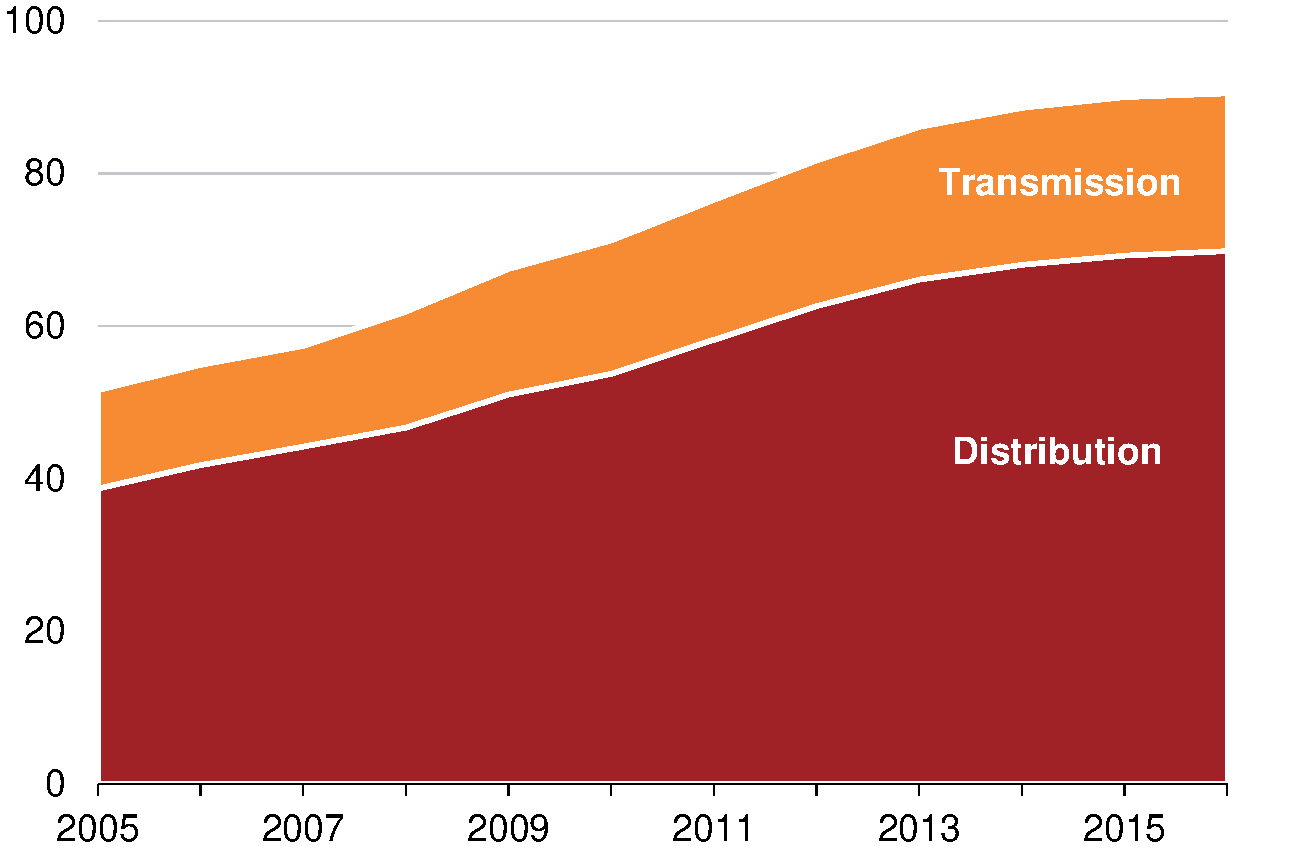
\includegraphics[page=1]{atlas/Charts.pdf}
\source{Grattan analysis of network determinations (\textcite{AER2018NetworkDeterminations}).}
\end{figure}

\section{Network assets have outgrown network use}\label{sec:network-growth-outgrown-usage}
There are some good reasons why more network infrastructure has been built over the past decade. There has been steady growth in the number of electricity customers in all states. Such growth requires extra expenditure by network businesses to connect people to the grid and ensure sufficient network capacity.

Total consumption of electricity has declined since the late-2000s,%
\footcite{AER2018NEMelectricityconsumption}
but \textit{peak} demand has grown, driven by the increase in customer numbers and greater use of air conditioning on hot days. The network needs to be big enough to cope at those times when consumers are using the most electricity. But growth in the RAB has far exceeded growth in customer numbers, demand or peak demand (see \Vref{fig:growth-in-network-assets-beats-usage}). 

\begin{figure}
\caption{Growth in network assets has far outstripped both potential use (capacity) and actual use}\label{fig:growth-in-network-assets-beats-usage}
\units{Change in distribution networks from a 2006 base, NEM-wide}
\includegraphics[page=2]{atlas/Charts.pdf}
\noteswithsource{`Network capacity' refers to the potential load (volts and amps) the network can handle. `Maximum demand' shown here is a NEM-wide aggregate of networks' peak demand, indicating the average change in maximum demand across networks.}{Grattan analysis of network determinations (\textcite{AER2018NetworkDeterminations}) and benchmarking data (\textcite{AER2017DNSPperformanceindicators}).}
\end{figure}

This report finds that network assets have outgrown usage -- a combination of customer numbers and peak demand -- by up to \$20 billion since RABs were initially valued in the late-1990s and early-2000s. The vast bulk of this `excess growth' or `over-investment' is concentrated in NSW and Queensland -- \$18.5 billion. 

The value of network assets per customer in NSW has increased from just over \$5,000 in 2006 to just under \$10,000 in 2016 (in real terms). In Queensland, assets per customer have increased from just under \$8,000 to almost \$14,000, and in Tasmania, from about \$7,000 to \$11,000 (see \Vref{fig:RAB-per-customer-over-time}).%
\footnote{`Per customer' includes both residential and business customers.}
By contrast, there has been little increase in Victoria and South Australia.

Some of the investment in NSW, Queensland and Tasmanian networks appears to be in over-valued or under-utilised assets -- either network businesses have paid too much for the infrastructure or the asset is bigger than it needs to be. Consumers will be paying for this historic over-investment for decades to come unless something is done.

\begin{figure}
\caption{The RAB per customer has skyrocketed in NSW, Queensland and Tasmania}\label{fig:RAB-per-customer-over-time}
\units{RAB per customer, 2017\$}
\includegraphics[page=24]{atlas/Charts.pdf}
\notewithsource{Initial valuation occurred at different times for different networks, ranging between 1995 and 2003. See the Technical Supplement to this report for more information.}{Grattan analysis of network determinations (\textcite{AER2018NetworkDeterminations}).}
\end{figure}

This report focuses on why the grid has grown so much, particularly in NSW and Queensland. It looks at the consequences of historic over-investment for consumers today, and makes recommendations on how best to deal with these legacy issues to reduce electricity bills and encourage efficient decisions about off-grid alternatives in future. 

\section{The size of the RAB largely determines network costs for consumers}\label{subsec:reg-model-for-networks}
The RAB reflects the value of the assets that network businesses have invested in on behalf of consumers. Network businesses are regulated monopolies, responsible for building and maintaining large amounts of expensive infrastructure with very long lives. In general, consumers do not pay for this infrastructure up front.%
\footnote{The exception is for the individual connection to the grid. For a household that does not have grid-based electricity, an up-front fee is required to connect the house with the main grid. The amount of this fee differs according to geography and the location of the house.}
Instead, the cost of building the network is paid for over the lifetime of the asset. 

Network businesses get the money back over time, plus a return on the investment that is used to cover the cost of debt and paying out dividends to those who have invested to build the infrastructure. An allowance for operating costs, which cover maintenance and staffing, is also charged to the consumer. 

Four main components determine the costs a network business can recover from customers each year: depreciation of network assets, the weighted average cost of capital (WACC), an allowance for operational expenditure (opex), and tax.%
\footnote{Network businesses also receive payments if they achieve efficiencies in their expenditure (or costs if they have been inefficient). But revenue derived through the Efficiency Benefits Sharing Scheme is currently a minor component of business revenue.}

Depreciation is where the consumer pays-off the value of the infrastructure. The WACC is the return to the network business for making that investment on behalf of consumers. These two components account for more than 60 per cent of the network costs passed through to consumers (see \Vref{fig:size-of-RAB-impacts-how-much-consumers-pay}).

\begin{figure}
\caption{The size of the RAB has a major impact on how much consumers pay}\label{fig:size-of-RAB-impacts-how-much-consumers-pay}
\units{Average share of distribution network revenue, 2017-18}
\includegraphics[page=5]{atlas/Charts.pdf}
\noteswithsource{Average across distribution networks. RAB = Regulated Asset Base; WACC = Weighted Average Cost of Capital; Opex = operational expenditure; Other = tax and revenue adjustments. Figures do not sum due to rounding.}{Grattan analysis of \textcite{AER2018NetworkDeterminations}.}
\end{figure}

As a result, the value of a business's infrastructure -- its Regulated Asset Base (RAB) -- has a major impact on the amount consumers pay. The bigger the RAB, the more consumers pay.

From a consumer's perspective, it's like a mortgage. The RAB is the unpaid balance of the mortgage. Depreciation is the principal paid on the balance, the WACC is the interest, and together they make up the mortgage repayment. Capital expenditure (capex) represents new borrowings to improve the house. The bigger the original value of the house, and the more you borrow to improve it, the bigger the mortgage repayment becomes.%
\footcite{AER2015consumerguide}

Network RABs were valued in the late-1990s and early-2000s when state electricity commissions were split up (see \Vref{box:privatisation-reforms}). RAB values have changed since, based on capital investments and depreciation. Growth of the RAB, particularly over the past decade, has been a major driver of network costs and consumer bill hikes in the National Electricity Market (NEM\@).%
\footnote{The NEM comprises Queensland, New South Wales, ACT, Victoria, South Australia and Tasmania. This report does not look at network costs in either Western Australia or the Northern Territory.}

\begin{bigbox}{Networks were split up and valued in the late-1990s}{box:privatisation-reforms}

\subsubsection{Networks became regulated monopolies in the 1990s}
Until the 1990s, electricity was delivered by government-owned, vertically integrated supply businesses that were responsible for the generation, transmission, distribution and retailing of electricity in each state and territory. In the 1990s, National Competition Policy reforms were introduced, following the 1993 Hilmer Review that encouraged competition in many industries including electricity.%
\footcite{Hilmer-1993-Review-Natl-Competition}

The state electricity commissions were split into generation, retail, transmission and distribution components. Transmission and distribution networks in each region became regulated monopolies. Victoria led the way, splitting its networks into five distribution companies (each covering a separate zone) and a transmission company, that were privatised in 1995. South Australia's network was privatised from 1998 to 2000. 

NSW split its network in 1995, but retained public ownership until very recently.%
\footnote{NSW's transmission network, TransGrid, remained government-owned until 2015. Two of the distribution networks, Ausgrid and Endeavour, became majority privately owned in 2016 and 2017, respectively. The third distribution network, Essential Energy, remains government-owned.}
The electricity sectors in Queensland and Tasmania were restructured in the 1990s but remain government-owned. 

Separate regulators in each state were initially responsible for setting network pricing, until the early-2000s when the ACCC took over regulation of transmission networks. By the late-2000s, the Australian Energy Regulator became the regulator for all networks in the NEM\@.

\subsubsection{How RABs were initially valued}
When network assets were valued in the late-1990s and early-2000s, Australian regulators accepted the depreciated optimised replacement cost (DORC) method in determining the size of RABs.%
\footnote{\textcite[][68]{AbbottTanKantor2014AssetValuation}. RABs were set largely based on DORC values but with government-led adjustments in some cases, discussed further in \Vref{box:impact-of-initial-RAB-valuations-on-estimate}. In our analysis we use the original DORC valuations rather than the adjusted valuations.}

The optimised replacement cost method values assets just short of the cost to a new entrant of providing the same service as the assets (system duplication), and therefore aims to emulate a contestable market. This value is then depreciated as per the age of assets, to get a DORC valuation.%
\footcite{Johnstone2003DORC}
Alternative valuation methods include the amount that assets cost when they were acquired, historical cost, or scrap value. DORC valuations tend to inflate asset book values relative to other methods, and DORC valuation is quite subjective.%
\footcites{Johnstone2001DORC}{Johnstone2003DORC}
Arguably, the fairest and most efficient valuation lies somewhere between scrap value and DORC but is impossible to pinpoint.%
\footcite{SAEconomics1998AssetValuation}

This report accepts the initial DORC valuations as the best available starting point for RABs. Although valuation was controversial at the time, networks in Victoria and South Australia were sold on the basis of these valuations and there is no other agreed estimate of the value of network assets. If anything, this should make our estimates of excess RAB growth conservative, because the original valuations were an upper-bound estimate.

\end{bigbox}

\section{Consumers are feeling the pain}\label{sec:consumers-feeling-the-pain}
Network costs are the biggest proportion of electricity bills for most customers in the NEM\@. For the average residential consumer, an estimated 42 per cent of the bill, or around \$700 a year, will be paid to network companies.%
\footnote{\textcite{ACCC2017ElectricityInterimReport}. ACCC estimates are for 2016-17, excluding GST, and are subject to further review and verification. The ACCC's average did not include Tasmania due to data quality issues.}

As well as being the largest component of the bill, network costs have also grown the most. Between 2007-08 and 2016-17, the network component of the bill increased 40 per cent on average across the NEM and was a major contributor to rising electricity bills, particularly in NSW and Queensland (see \Vref{fig:network-costs-biggest-contributor-to-bill-growth}).%
\footnote{\textcite{ACCC2017ElectricityInterimReport}. The ACCC figures for 2016-17 are estimates, but the 2015-16 figures are higher. In South Australia, wholesale costs were the largest growth component, followed by networks (\textcite{ACCC2017ElectricityInterimReport}). In Victoria, retail costs were the largest growth component (\textcites{ACCC2017ElectricityInterimReport}{WoodBlowers-2017-Price-shock}).}
In Tasmania, network costs have been relatively steady since 2011, but grew 60 per cent in the decade prior.%
\footnote{On a cents per kilowatt hour basis (see \textcites{Tas2011PriceTrends}{AEMC2013PriceTrends}{AEMC2017PriceTrends}).}

Growth in the value of network assets was not accompanied by similar growth in customer numbers or peak demand. The result was that electricity consumers paid more and more for their connection to the grid.

Network costs are now starting to come down,%
\footnote{Revenue allowances are lower for the current determination period than the previous one. The AER sets a network business's revenue allowance for a five-year period based on the expected efficient costs of running that network over the period. This process is known as a network determination.} 
but remained the largest component of the bill in all states in 2016-17%
\footnote{\textcite{AEMC2017PriceTrends} shows network costs are the largest component of the bill in all states including Tasmania. \textcite{ACCC2017ElectricityInterimReport} estimates show wholesale costs exceeding network costs in South Australia in 2016-17.}
and are still higher than a decade ago. And consumers are still paying, through their bills, for the historic over-investment in the network.

\begin{figure}
\caption{Network costs were the single biggest contributor to bill growth over the past decade in NSW and Queensland}\label{fig:network-costs-biggest-contributor-to-bill-growth}
\units{Change in average residential bill, 2007-08 to 2016-17, 2015-16\$}
\includegraphics[page=4]{atlas/Charts.pdf}
\noteswithsource{Real values in 2015-16 dollars. In South Australia, wholesale costs grew more than network costs. In Victoria, retail and smart-meter costs grew more than network costs (although smart meters are paid for through the network tariff). Data is from the ACCC's preliminary report on retail electricity pricing and is subject to further review and verification (for example, SA Power Networks contests the size of the network component in South Australia and has raised the issue with the ACCC)}{Grattan analysis of \textcite{ACCC2017ElectricityInterimReport}.}
\end{figure}

Beyond the immediate hit to the hip pocket, excessive network costs have broader consequences for the future of the grid. An overly-expensive network can change people's choices about staying `on the grid' or going `off-grid' for part of or all their energy needs.%
\footnote{The way network costs are reflected in network tariffs also influences people's choices, discussed further in \Chapref{chap:looking-forward-to-prevent-this-happening-again}.}
Excessive network costs will encourage a greater take-up of solar PV, batteries and back-up diesel generation (for those who can afford it) than if costs reflected the `real value' of the network.

The risk with inefficient adoption of distributed generation is that total costs go up. Consumers who can afford it invest in distributed generation and reduce their grid use, while those who cannot end up paying more for the same assets.

\section{Future unknown}\label{sec:future-unknown}
Major changes have been made since the high capital expenditure of 2005-2014. The regulatory framework has been improved,%
\footcite{AER2014betterregulation} and most of the network businesses in NSW have been either fully or partially privatised. 

Given these changes, the high expenditure of 2005-2014 should be treated as a legacy issue. But this does not mean that the regulatory processes are perfect. Nor that this legacy issue can be swept under the carpet.

New challenges are arising and the legacy of over-investment could make dealing with these challenges more difficult. The energy system is transforming, away from a centralised, fossil-fuel dominated electricity sector. It is hard to know what the future grid will look like, but it could be very different from today's model. The nature of renewables means that generation is likely to be more distributed. More and more households are choosing to generate their own power. Solar may be coupled with battery storage to allow households to become energy self-sufficient. 

It is likely that some grid infrastructure could become `stranded' in future and that some will be used differently. As large-scale generation moves away from its traditional home in places like the Latrobe and Hunter valleys, infrastructure that transported electricity from those regions will no longer be needed. And electricity no longer flows in one direction -- from big, central power stations, through transmission and distribution networks, to homes and businesses. As more consumers generate their own power, and some communities separate from the main grid, parts of the distribution network may be used differently or not needed at all.

Dealing with the future risk of stranded assets is a different issue to dealing with the legacy of over-investment in the grid. Assets will be stranded in future as a result of fundamental changes in technology and demand. Continuing to pay for legacy over-investment through consumer bills could hinder the transition now underway in Australia's energy system. Consumer preferences should guide the transition, but network (and other) costs need to be allocated efficiently so that consumer preferences encourage efficient future investments.

\Chapref{chap:history-how-we-got-here} of this report looks at why so much network infrastructure has been built over the past decade, particularly in NSW and Queensland.

\Chapref{chap:a-more-sustainable-RAB} estimates the amount of excessive RAB growth that has occurred.

\Chapref{chap:whose-fault} looks at who was responsible for driving over-investment in the grid. 

\Chapref{chap:looking-back-write-down} explains why policy makers should not ignore the legacy of over-investment, and makes recommendations on how to remove that over-investment from the RAB\@.

And \Chapref{chap:looking-forward-to-prevent-this-happening-again} explores the challenge of dealing with future stranded assets, recommends policies to mitigate this risk, and identifies areas for future work.



\chapter{How we got here}\label{chap:history-how-we-got-here}

Capital expenditure ballooned between 2005 and 2014, particularly for NSW and Queensland distribution networks (see \Vref{fig:capex-by-state-over-time}). For most of this period, capital expenditure allowances were higher than they had been historically, and all capital investment by network businesses, including expenditure above allowances, was rolled directly into RABs. Capital expenditure allowances have since been reeled in by the AER, in the most recent round of determinations, and new incentives to improve the efficiency of capital expenditure were introduced in 2013.%
\footcite{AER2013capexincentives}

There are several reasons for such high capital expenditure, including: the underlying incentive structure for network businesses; public ownership; high reliability standards; fluctuations in demand; and replacement of ageing assets. But while these reasons collectively may explain the capital expenditure, they do not \emph{justify} so much investment in such a short time. 

\begin{figure}
\caption{Capital expenditure ballooned between 2005 and 2014}\label{fig:capex-by-state-over-time}
\units{Annual capex, 2017\$ billions}
\includegraphics[page=33]{atlas/Charts.pdf}
\notewithsource{Distribution networks only.}{Grattan analysis of network determinations (\textcite{AER2018NetworkDeterminations}).}
\end{figure}


\section{Some networks grew far more than others}\label{sec:some-networks-grew-more-than-others}

The rise and fall of capital expenditure in NSW and Queensland stands out. NSW and Queensland distribution networks grew most -- whether measured in absolute terms, percentage terms, or per customer (see \Vref{fig:RAB-per-customer-absolute-and-percent}).

Capital expenditure also increased for networks in Victoria, South Australia, Tasmania and the ACT, but more steadily. The increase in Victoria from 2009 to 2014 was partly to meet demand and partly due to the introduction of safety requirements after the 2009 bushfires.%
\footnote{Additional capex was approved for the regional distribution networks, AusNet and Powercor, to replace overhead lines in bushfire-prone areas. These measures resulted in at least \$600 million in additional safety-driven capex between 2009 and 2015 (\textcite{AER2010VICDistributionFinalDetermination}).}

\begin{figure}
\caption{NSW and Queensland assets grew far more than most, per customer, since 2005-06}\label{fig:RAB-per-customer-absolute-and-percent}
\units{Change in RAB per customer 2005-06 to 2015-16, in 2017\$ and per cent}
\includegraphics[page=25]{atlas/Charts.pdf}
\noteswithsource{D = distribution, T = transmission.}{Grattan analysis of network determinations (\textcite{AER2018NetworkDeterminations}).}
\end{figure}
 
% \begin{figure}
% \caption{NSW and Queensland assets grew far more than most, per km of line, since 2005-06}\label{fig:RAB-per-km-absolute-and-percent}
% \units{Real change in RAB per km of line, in \$, and in per cent}
% \includegraphics[page=26]{atlas/Charts.pdf}
% \noteswithsource{2017 dollars. Growth per km of line is larger for transmission networks than distribution networks because distribution networks have substantially greater circuit line length.}{Grattan analysis.}
% \end{figure}


\section{Five main reasons for over-investment}\label{sec:reasons-why}
There are five main hypotheses to explain the high capex from 2005-2014:
\begin{enumerate}
 \item Incentive structure: a high WACC may have encouraged over-investment;
 \item Ownership: publicly-owned businesses have a greater incentive to spend more;
 \item Higher expectations: new reliability and safety standards were imposed;
 \item Changing demand: usage was expected to grow more than it actually did; and
 \item Cycles of investment: asset replacement can be lumpy over time, so high investment in one period may be `catch up' for previous under-investment.
\end{enumerate}

All appear to have played a role, to different degrees in different states. But ownership, reliability standards and changing demand appear to have been particularly important in driving investment in NSW and Queensland networks where most of the RAB growth occurred.

\subsection{Incentive structure}\label{subsec:incentive-structure}
A high WACC may have encouraged over-investment. The regulator sets the WACC for network businesses to recover their costs of capital: cost of debt and cost of equity. Historically the costs of debt and equity appear to have been set too high for distribution businesses.%
\footnote{See \textcite{WoodHunterOTooleEtAl2012}. Additionally, the recent sales of TransGrid and part of Endeavour for 1.7 times RAB value suggests abnormally high returns, when utilities typically sell for 1.3 times RAB value (\textcites{AFR2016AusgridPrice}{Morgans2017UtilitiesSales}).}

Arguably the regulator will always err on the side of caution, allowing a higher WACC\@. If the WACC is too low, businesses will not invest because they cannot recover their financing costs. A risk-averse regulator that seeks to minimise the risk of blackouts is likely to slightly overestimate the costs of both debt and equity. 

The immediate impact of a high WACC is to increase costs for consumers. But setting these costs too high over time may also create an incentive for over-investment, because money will chase above-market returns. 

\begin{figure}
\caption{WACC levels were very high until recently}\label{fig:WACC-high-until-recently}
\units{}
\includegraphics[page=8]{atlas/Charts.pdf}
\noteswithsource{Distribution networks only, 2002-2016, except Tasmania where the WACC has now been set for 2018. WACC levels are typically set at the start of a determination period, and hold for the next five years. A high WACC was set in the 2009 and 2010 determinations in most states, after the GFC, but the Tasmanian determination came later, in 2012, by which time financial market conditions had changed. WACC levels for Victoria are averaged across the five networks.}{Grattan analysis of network determinations (\textcite{AER2018NetworkDeterminations}).}
\end{figure}

The WACC was particularly high in the late-2000s, when most of the capital expenditure occurred (see \Vref{fig:WACC-high-until-recently}). A high WACC was justified on the basis of higher debt costs following the Global Financial Crisis. But given significant investment during that period, it appears the WACC was more than sufficient. 

The WACC is calculated in the same way for all network businesses. So if a high WACC was solely responsible for increased investment, there would have been excessive capital expenditure across all networks. Yet businesses in South Australia and Victoria did not grow nearly as fast as those in Queensland and NSW\@.

\subsection{Ownership}\label{subsubsec:incentive-structure-plus-ownership}
Networks in Queensland and Tasmania are publicly-owned, and NSW networks were too until very recently. Growth in RAB per customer of publicly-owned networks far outstrips growth in privately-owned networks (see \Vref{fig:Public-v-private-RAB-per-customer}).

\begin{figure}
\caption{Public networks grew far more than private networks}\label{fig:Public-v-private-RAB-per-customer}
\units{RAB per customer, 2017\$}
\includegraphics[page=27]{atlas/Charts.pdf}
\noteswithsource{Three of the four NSW networks were partially or fully privatised from 2015 to 2017, but are counted here as public networks because growth in RAB occurred while they were publicly-owned. Initial valuation occurred at different times for different networks, ranging between 1995 and 2003.}{Grattan analysis.}
\end{figure}

Analysis of Australian government-owned electricity distribution businesses also showed that, compared to private distribution businesses and international benchmarks, government-ownership coupled with the regulatory regime led to over-investment in assets.%
\footcites{Mountain2017PhD}{Mountain2018NetworkArticleInPress}

There are a number of reasons why public ownership of network businesses can lead to higher costs.

First, the government has a conflicted role as both owner and rule-maker. As owner it may want to maximise revenues, and as government it can set rules to achieve this. It may seem politically easier to raise additional government revenue through electricity profits than through additional taxes.%
\footnote{Of course additional electricity profits are a much less economically efficient way to raise additional revenues, but the primary drivers in this scenario are political not economic.}
Reliability standards or other regulatory interventions are less politically visible and contentious than tax rises.%
\footnote{This was probably true in the mid-2000s, even if this political calculus is changing with growing public concern about electricity prices.}
% By contrast, government is more likely to be critical of proposals that will increase costs if it is the regulator but \emph{not} the owner of electricity assets.

Second, a government owner may be less concerned about over-building than a private owner. The government has a say in the regulatory regime that determines whether investments can be recouped. 

Third, a government owner may be tempted to promote additional building to improve reliability, over and above the regulatory standards. Governments tend to be extremely averse to the risks of even minor outages.

Fourth, a government owner may have other non-profit motives for additional construction, such as a desire to boost economic growth, or to train additional apprentices.%
\footcites{WoodHunterOTooleEtAl2012}{Mountain2017PhD}
It may also have non-profit motives for procurement and employment policies that can mean higher costs in providing the same infrastructure than a privately-owned business.
\footcite{PC2013ElectricityInquiry}

Finally, governments can borrow more cheaply than private providers, but consumers do not directly reap the benefit; instead, the difference goes to the state. Publicly-owned businesses pay `competitive neutrality' fees to the state that are intended to put them on equal terms with a private business. This means the more money a publicly-owned distribution business spends on infrastructure, the higher the `competitive neutrality' fee paid to state government.%
\footcite{WoodHunterOTooleEtAl2012}


% There are a number of reasons why public ownership of network businesses can lead to higher costs. In particular, the fact that the government has a conflicting role as both shareholder and financier, and that there may be interference in publicly-owned businesses to deliver political outcomes.%
% \footcites{WoodHunterOTooleEtAl2012}{Mountain2017PhD}
% A publicly-owned business might have a bias towards reliability or job creation over cost, for example. 
 
% The regulator allows publicly-owned businesses a rate of return equivalent to the cost of debt available to private providers. But because the cost of debt for government is lower than for private providers, state-owned businesses also pay `competitive neutrality' fees intended to put them on equal terms with a private business. The state, as both the owner and financier, benefits either way, because networks do not compete directly with any other business, and the fees are paid straight to the state government. The more money a publicly-owned distribution business spends on infrastructure, the higher the `competitive neutrality' fee paid to state government. 
% % The `competitive neutrality' fee increases the overall cost of service provision, penalising consumers. 

% The potential incentive for government-owned businesses to spend more on their networks depends on the degree of separation in the state government's dual roles as shareholder and financier.%
% \footcite{WoodHunterOTooleEtAl2012}
% If the `Chinese walls' between the network business and the treasury are effective, the outcome for a publicly-owned business should be the same as for a privately-owned business. But if those walls break down, then government-owned businesses may have an incentive to spend more. 

% Analysis of Australian government-owned electricity distribution businesses shows that, compared to private distribution businesses and international benchmarks, government-ownership coupled with the regulatory regime has driven over-investment in assets.%
% \footcites{Mountain2017PhD}{Mountain2018NetworkArticleInPress}

% Government owners also face political pressures that private companies do not. These include procurement and employment policies that can mean higher costs in providing the same infrastructure as a privately-owned business.%
% \footcite{PC2013ElectricityInquiry}
% And above all, politicians are held accountable for blackouts, so there is political pressure to give priority to reliability. This creates the potential for political interference in the operations of government-owned companies. 

These differences offer some explanation for why publicly-owned networks outgrew privately-owned networks (see \Vref{fig:Public-v-private-RAB-per-customer}). But the extent of the impact of each is difficult to quantify. 

\subsection{Reliability and safety standards}\label{subsec:reliability-standards}
The Queensland and NSW Governments introduced new reliability standards for distribution networks in 2005, after power outages in 2004.%
\footnote{In Queensland, extended network outages due to storms and extreme heat in 2004 led to a major review of the networks that recommended immediate upgrades (\textcite{Somerville2004EDSDreview}). In NSW, a few short but high-profile outages in Sydney appear to have prompted reforms (\textcite{Maley2004SydneyBlackouts}).}
Significant investment in Queensland and NSW networks followed (see \Vref{fig:capex-over-time}), some of which can be directly attributed to the introduction of the standards. 

\begin{figure}
\caption{Investment in NSW and Queensland networks increased substantially after new reliability standards were introduced in 2005}\label{fig:capex-over-time}
\units{Capex, 2017\$ billions}
\includegraphics[page=6]{atlas/Charts.pdf}
\noteswithsource{AGD = Ausgrid (NSW), ERG = Ergon Energy (QLD), ENX = Energex (QLD), ESS = Essential Energy (NSW), TRG = TransGrid (NSW), END = Endeavour Energy (NSW), and PWL = Powerlink (QLD). Transmission networks, TransGrid and Powerlink, were only indirectly affected by the reliability standards for distribution networks (in that they were obliged to ensure distribution networks could meet their obligations).}{Grattan analysis of network determinations (\textcite{AER2018NetworkDeterminations}).}
\end{figure}

The reliability standards introduced in NSW were highly-prescriptive and legally-binding -- specifying inputs, not just outputs. For example, Ausgrid had to meet an \emph{N-2} security-of-supply requirement for the Sydney CBD\@. An \emph{N-2} standard required the network to have sufficient redundancy to avoid power supply interruptions if any two elements in the system failed. The standards were set without reference to the value customers place on reliability.%
\footcite{IPART2016ReliabilityStandardsReview}
NSW distribution networks had to apply for additional expenditure (both opex and capex) in 2005 to meet the new requirements. Additional capex of \$1.8 billion was approved as a direct result and a further \$1.6 billion was approved for reliability in the following determination.%
\footnote{In 2017 dollars, for the 2004-05 to 2008-09 determination and the 2009-10 to 2013-14 determination, respectively (\textcite{IPART2006statementofreasons} and \textcite[][119]{AER2009NSWDistributionFinalDetermination}).}

In Queensland, the reliability standards required Energex and Ergon Energy to achieve incremental \emph{improvements} in network reliability over time.%
\footcite{QCA2013ReliabilityStandardsReview}
This led to an extra \$3 billion in capex allowed between 2005-06 and 2009-10.%
\footnote{Above historical capex levels, and specifically attributed to the 2004 review.}
Networks exceeded their allowances by \$2 billion, and this was added to their RABs in the following determination. The new, higher capex levels were maintained in the next determination and only began to decline very recently.
Reliability standards in both Queensland and NSW were later found to be excessively cautious, but not before they had driven significant capital expenditure.%
\footcites{PC2013ElectricityInquiry}{Bellas2014IRPonnetworkcosts}

% In Victoria, new safety requirements after the 2009 bushfires drove the need for increased capital expenditure in the following period. The Victorian Bushfires Royal Commission recommended enhanced safety standards for electricity distribution businesses, and the state government introduced other electrical safety requirements around the same time. The AER approved additional capex for the regional networks, AusNet Services and Powercor, to replace overhead lines in bushfire-prone areas.%
% \footcite{AER2010VICDistributionFinalDetermination}
% These measures resulted in at least \$600 million in additional safety-driven capex between 2009 and 2015.%
% \footcite{AER2010VICDistributionFinalDetermination}

\subsection{Changing demand}\label{subsec:changing-demand}
Maximum demand is a major driver of network costs, and networks often (but not always) need to build in advance of expected increases in maximum demand. But in the mid-to-late 2000s, actual maximum demand fell well short of expected maximum demand as forecast in five yearly regulatory determinations.%
\footnote{Grattan analysis of maximum demand forecasts reported in regulatory determination processes between 2006 and 2015 for distribution networks in NSW, Queensland and Victoria.}
Getting the forecasts so wrong is likely to have contributed to some of the over-investment. 

Yet even if businesses had built according to expected maximum demand, rather than actual maximum demand, this would not explain all the RAB growth in NSW and Queensland (see \Vref{fig:network-growth-exceeded-expected-demand}). And other networks would have substantially larger asset bases had they grown in line with maximum demand as expected in regulatory determinations. This indicates at least some networks reduced their expenditure programs once demand proved to be less than forecast.

\begin{figure}
\caption{RAB growth even exceeded expected demand for many distribution networks}\label{fig:network-growth-exceeded-expected-demand}
\units{Average annual growth, 2006-2014}
\includegraphics[page=7]{atlas/Charts.pdf}
\noteswithsource{Demand growth is both customer numbers and maximum demand; or, where maximum demand was negative, then it is customer growth only. JEN = Jemena, CIT = Citipower, PCR = Powercor, AND = AusNet distribution, UED = United Energy, ESS = Essential, AGD = Ausgrid, END = Endeavour, ENX = Energex, and ERG = Ergon}{Grattan analysis of expected demand in past determinations and actual demand based on AER benchmarking data.}
\end{figure}

\subsection{Cycles of investment}\label{subsec:cycles-of-investment}
Asset replacement cycles drive periods of higher and lower investment. Capital expenditure can be particularly `lumpy' for electricity transmission because of the nature of the assets. 

If network investment did not keep pace during a period of rapid growth in demand in the early-2000s, then additional expenditure may be required in the late-2000s to `catch-up' -- augmenting or replacing infrastructure under strain. 

This appears to have been an important factor in Queensland, where a 2004 review of networks found that Queensland's urban distribution network, Energex, had been under-investing in assets and this was compromising reliability.%
\footcite{Somerville2004EDSDreview}
One reason was an earlier switch from peak demand occurring in winter, to peak demand occurring in summer, mainly because air conditioners were used more. The same peak demand requires more capacity in summer because heat reduces the effective capacity of the network.%
\footnote{\eg{ \textcite{Sathaye2012CaliforniaRisktoEnergyInfrastructure}}.}

The review's findings drove significant capital investment over the following two determinations, through the introduction of reliability standards that were later found to be inefficient.%
\footcite{Bellas2014IRPonnetworkcosts}
Some component of this expenditure appears to have been `catch-up', but is difficult to distinguish from expenditure associated with the overly-prescriptive standards. Exactly how much was needed will depend on asset utilisation today.

Asset age can be an indicator of historical under-investment; an older fleet might imply that replacement expenditure did not keep pace with need over time.%
\footnote{But there is no `ideal' fleet age, because different assets have different lifetimes, and networks may estimate this in different ways.}
In 2006 (prior to most of the expenditure), the average residual life of assets ranged from 17 to 38 years, depending on the network.%
\footnote{Residual life of assets is reported by network, by asset class (\textcite{AER2018NetworkPerformanceRINResponses}). The average residual life of assets for each network is the average across all asset classes, weighted by the value of each asset class. Networks self-reported this data and it appears that they have reported the number of years remaining to pay off the asset rather than the number of years that assets are expected to remain in service (which could be longer).}
Surprisingly though, networks \emph{younger} than the NEM average of 25 years spent \emph{more} in the following years than older networks. For individual networks, asset age may have been a factor, but the available information does not point to asset age as a major driver of capital expenditure (\Vref{fig:asset-age-vs-capex}).%
\footnote{See Technical Supplement for further discussion.}

\begin{figure}
\caption{There is no consistent trend to suggest asset age is a major driver of capital expenditure}\label{fig:asset-age-vs-capex}
\units{LHS = Total capex 2006-2014 (as a per cent of 2006 RAB); RHS = Remaining life of assets in 2006 (years)}
\includegraphics[page=39]{atlas/Charts.pdf}
\noteswithsource{This chart compares the remaining life of assets (in red) as at 2006 (before most investment occurred) to total capital expenditure per customer over the following years (in orange). The average residual life of a networks assets is the residual service life by asset class, weighted by asset value. PCR = Powercor, SPN = SA Power Networks, UED = United Energy, CIT = Citipower, ESS = Essential, TND = TasNetworks distribution, ERG = Ergon, PWL = Powerlink, TRG = TransGrid, ACT = ActewAGL, JEN = Jemena, ENX = Energex, ELN = ElectraNet, ANT = AusNet transmission, AND = AusNet distribution, AGD = Ausgrid, TNT = TasNetworks transmission and END = Endeavour}{Grattan analysis of actual capex in network determinations (\textcite{AER2018NetworkDeterminations}) and residual life of assets reported by networks (\textcite{AER2018NetworkPerformanceRINResponses}).}
\end{figure}

It appears many networks undertook substantial asset augmentation and replacement programs at a time when material and labour costs were high.%
\footnote{According to Energy Networks Australia, newer assets are relatively more expensive due to modern environmental and safety standards, and a constrained supplier market.}
The average age of assets at the time would suggest much of this was premature. While high-cost asset augmentation and replacement may explain some of the over-investment, it is not clear that so much was needed in such a short time. 


\section{Legacy over-investment was still excessive}\label{sec:growth-still-excessive}
Investment was clearly driven by many factors. Major RAB growth in public networks, compared to minimal growth in private networks, implies very different incentives for different kinds of ownership. 

Some of the drivers of capex were out of network businesses' control. Externally-imposed reliability standards that specified inputs not just outputs, such as those in NSW and Queensland, required significant additional expenditure.

Each network has its own specific reasons for the capital investments that were made. And these investments were approved by the regulator at the time. The problem is that consumers can't and shouldn't pay more and more for the same service -- it is unsustainable.

Productivity measures that compare the cost of the network (capex and opex) with the services delivered (such as meeting demand for electricity, and reliability) show that productivity has declined since measurement began in 2006, with only a slight uptick in 2016.%
\footcite{AER2017BenchmarkingReport}

In a system that is supposed to work for consumers, it is remarkable that so much capital expenditure was allowed in such a short time. The National Electricity Objective (which has been in place since 2005) clearly prioritises \emph{efficient} investment in and operation of electricity services for \emph{the long-term interests of consumers}.%
\footnote{\textcite{AEMC2018NationalElectricityObjective}, our emphasis.}

RAB growth cannot outstrip usage for too long before it becomes unaffordable for consumers and undermines the business model of networks. RAB growth might exceed use in some years, but this should even out with lower growth in other years. An asset base that outgrows demand, over a period of a decade or more, is unsustainable.



\chapter{A more sustainable RAB}\label{chap:a-more-sustainable-RAB}

There is no definitive way to measure an efficient RAB or efficient investment. If it was easy to define, over-investment probably wouldn't have happened in the first place. This chapter describes what a more sustainable RAB would look like.

A good starting point is usage. It is not a direct determinant of costs but it is a simple indicator of the value consumers place on network assets and how this value has changed over time. A more sustainable rate of RAB growth would be one in line with network usage.

Ultimately existing assets must be paid for, but there are various options for who pays for them and how. In attempting to determine the size of a more sustainable RAB, we aim to determine how much the consumer should be paying for through their existing network tariff. How the remainder (the `excess' portion) is paid for is discussed in \Chapref{chap:looking-back-write-down}.

\section{RABs should grow in line with usage}\label{sec:RABs-should-grow-in-line-with-usage}

For network assets to be sustainable in the long run, growth in asset values needs to be in line with growth in use of the network. When real asset growth exceeds use, consumers end up paying more without receiving additional value.%
\footnote{Except where the value to the consumer is in reduced wholesale prices, as with some transmission developments, discussed in \Chapref{chap:looking-back-write-down}.}
This might be bearable for a short time, but not in the long run.%
\footnote{For example, \textcite{simshauser2017monopoly} argues `persistent electricity tariff increases above general inflation rates will eventually prove problematic'.}

Usage is not a direct determinant of costs. A 5 per cent increase in maximum demand or customer numbers will rarely translate directly to a 5 per cent increase in RAB\@. Even so, growth in use should serve as the upper bound for asset growth, because real asset growth greater than use over the long term is unsustainable for the customer and therefore for the business too. Over time, consumers spend more of their income on network services, and eventually they are unable to afford grid-based electricity, and so must find alternatives. Network businesses suffer as a consequence.

If a network's assets are growing at the same rate as its customer base, then the cost per customer remains constant. If customers increase usage, particularly at peak times, then it is reasonable that they pay more to cover the increased costs they are placing on the grid.%
\footnote{We note though that most consumers do not yet face cost-reflective pricing, so are unlikely to be aware of their contribution to maximum demand and grid costs. It is possible that maximum demand would be lower if consumers faced efficient prices.}
The network is built to meet maximum demand. We therefore estimate efficient asset growth, on par with actual use, as growth in line with both customer numbers and maximum demand (see \Vref{box:methods-and-data}). We consider asset growth above this to be `excessive'.


\begin{bigbox}{How we estimate excessive growth}{box:methods-and-data}

For this report we use regulatory determinations to assess total growth in assets by network. We then compare the growth of each network's RAB to growth in usage of that network. We allow for RABs to grow, in real terms, by the same percentage as growth in network use. Any RAB growth above this we consider to be `excessive'. 

\subsubsection{How we define network use}
We define `network use' as the aggregate of growth in customer numbers and growth in maximum demand.%
\footnote{We use coincident maximum demand for most networks, because this was reported historically. Maximum demand is reported net of exports so may exclude some transmission capacity that supports interconnectors. We allow for this in our recommendations (\Chapref{chap:looking-back-write-down}).}
For example, a 1 per cent increase in each equates to a 2 per cent increase in `network use', so the RAB can increase by 2 per cent to stay on par with `network use'.%
\footnote{Where change in maximum demand is negative, it is treated as zero (\ie{ negative growth in one type of usage does not discount growth in another}).}

This whole-of-network measure obscures the possibility that some parts of a single network might be growing while others are shrinking. We deliberately choose this measure because shrinking demand represents under-utilised assets. But we recognise that maximum demand might be low in one year and then high in the next. For this reason, we use the highest maximum demand of the past five years in assessing appropriate growth.

Network use is a simple measure, representing the upper limit for reasonable RAB growth. It may \emph{overestimate} the actual need for RAB growth, because maximum demand is likely to be a function of increasing customer numbers. RAB growth above network use is unsustainable unless accompanied by radical improvement in other services, such as reliability, that customers genuinely value.

Transmission networks serve both consumers and generators. We therefore considered using an alternative measure to customer numbers that captures both consumers and generators (see the Technical Supplement to this report). But given that the AER now uses customer numbers as the key output measure for transmission, we do the same.%
\footcite{AER2017TNSPperformanceindicators}

\subsubsection{Starting point for growth analysis}
Our analysis starting point ranges from 1996 to 2005-06, depending on the network. The starting point is when a network's RAB was initially valued, or as early as publicly available data allow. 

Differing starting points enabled us to conduct the longest possible analysis for each network. A longer time frame is preferable because it encompasses more of the asset replacement cycle (see \Cref{subsec:cycles-of-investment}). 

Our estimate of excess growth is based on change in RAB compared to change in usage within a network, so does not depend on all networks sharing a common time-frame of analysis. Our analysis assumes that all states had an efficient network asset base at the time of the initial DORC valuations.%
\footnote{Networks in Victoria and South Australia were sold on the basis of these valuations and there was no other agreed estimate of asset size at the time. Asset values since have been rolled-forward from these original valuations.}
The implications of this assumption are discussed further in \Vref{box:impact-of-initial-RAB-valuations-on-estimate}.
One network, Energex, provided data on historic under-investment prior to the analysis window, so for this network a range estimate is provided.

For further information on our methodology and data sources, see the Technical Supplement to this report.

\end{bigbox}


\section{How much is `excessive'}\label{sec:how-much-is-stranded}
If we take the longest possible view -- going back as far as public data will allow -- RABs have outgrown network use by about \$20 billion. A longer view is preferable because of the lumpy nature of capital expenditure; a period of high expenditure may be followed or preceded by a period of low expenditure (see \Vref{subsec:cycles-of-investment}). Over 15-to-20 years this should even out, but over the past 15-to-20 years it has not.

RAB growth of \$20 billion above network use has locked in additional costs for current and future consumers, without delivering additional value. Consumers may be willing to pay more if today's network offered a radically improved service, but it is hard to see much evidence of such improvement. Exactly how much spending was excessive depends on how much network services have improved over time and how much value consumers place on these improvements. While the reliability of some networks has improved, the degree of improvement does not justify a spending increase of this size (see \Vref{sec:what-should-consumers-pay-for}). 

Our estimate covers three very different kinds of excessive growth:
\begin{enumerate}
 \item Poles going nowhere: These are genuine stranded assets in the sense that they can no longer be used at all. For example, the transmission lines that connect a major generation region to the grid may become stranded when generators in the region close.%
 \footnote{The owner of a generator usually pays for the most immediate infrastructure that connects them to the grid, but transmission lines to the region tend to be shared assets, paid for by consumers. The location and size of shared transmission infrastructure will need to change as the generation mix changes, leaving some existing assets unused.}
 \item Overcapacity: This includes larger substations and transformers than are actually required today. Additional capacity might have been built to meet demand in the past, or expectations of demand, but if that demand is no longer likely to eventuate, then even though the line is still in use, the additional capacity is excessive.
 \item Inefficient expenditure: This includes upgrades and additions that could have been delayed, or where cheaper alternatives were available.
\end{enumerate}

There are unlikely to be many assets in the first category for now, because only a few generators have been retired, and very few communities have separated entirely from the grid. But we would expect there to be more stranded assets of this kind in future.

Most of the excessive growth we have identified is likely to fall into the other two categories -- overcapacity and inefficient expenditure. In this sense they are not truly `stranded' assets, but under-utilised and over-valued assets.

A more precise estimate of under-utilised and over-valued assets in the NEM would require detailed network data on asset utilisation (which are not in the public domain) and considerable resources. Even then, some judgment would still be required in assessing the availability of alternative investments in the past and the potential for assets to be useful in future. For these reasons we have not attempted to develop a bottom-up estimate of under-utilised and over-valued assets, but instead provide a top-down `sense check' on past RAB growth.%
\footnote{Our recommendations in \Chapref{chap:looking-back-write-down} allow for adjustments to be made to our estimate on the basis of current asset utilisation levels and expected future demand. This means that if significant under-investment (or over-investment) occurred prior to the analysis period it should be reflected in asset utilisation levels today and can be taken into account.}


\section{How excessive RAB growth is distributed}\label{sec:how-stranded-assets-are-distributed}
Our analysis suggests that the NEM's \$90 billion RAB is unsustainably high, and that a more sustainable RAB would be up to \$20 billion or 22 per cent lower.

Excessive RAB growth is highly concentrated in NSW and Queensland networks, with \$18.5 billion of excessive growth in these two states alone. The seven networks in NSW and Queensland together represent 71 per cent of today's RAB and 92 per cent of the excessive growth (see \Vref{fig:size-of-stranded-assets}).

\doublecolumnfigure{
\caption{Network assets are over-valued by up to \$20 billion based on network use}\label{fig:size-of-stranded-assets}
\units{Excessive growth by state, 2017\$ billions}
\includegraphics[page=9]{atlas/Charts.pdf}
\notewithsources{See \Vref{box:methods-and-data} and Technical Supplement for our methodology.}{Grattan analysis of network determinations (\textcite{AER2018NetworkDeterminations}), performance data (\textcites{AER2017DNSPperformanceindicators}{AER2017TNSPperformanceindicators}{AER2018NetworkPerformanceRINResponses}) and historic reports.}
}{
\caption{Assets outgrew use far more in some networks than others}\label{fig:excess-growth-by-network}
\units{Excess RAB growth, 2017\$ billions}
\includegraphics[page=21]{atlas/Charts.pdf}
\noteswithsources{AGD = Ausgrid, ESS = Essential, TG = TransGrid, END = Endeavour, ENX = Energex, ERG = Ergon, PL = Powerlink, EL = ElectraNet, T = TasNetworks transmission, D = TasNetworks distribution, JEN = Jemena, CIT = Citipower. For the remaining networks not shown, RABs grew less than network usage. A range is provided for Energex based on data provided by Energex about capital under-investment prior to the analysis period. See Technical Supplement for more information.}{Grattan analysis of network determinations (\textcite{AER2018NetworkDeterminations}), performance data (\textcites{AER2017DNSPperformanceindicators}{AER2017TNSPperformanceindicators}{AER2018NetworkPerformanceRINResponses}) and historic reports.}
}

When the \$750 million excess in Tasmania is included, the publicly-owned networks represent 76 per cent of today's RAB, and 96 per cent of the excessive growth.%
\footnote{Three networks in NSW were publicly-owned at the time but have recently been privatised. TransGrid, Ausgrid and Endeavour were wholly or majority privatised in 2015, 2016 and 2017 respectively.}
Most of the excessive growth is in distribution (81 per cent), rather than transmission (19 per cent).

There are further differences between the individual networks. In all networks in NSW, Queensland and Tasmania, RABs outgrew usage; in some, RABs outgrew usage by more than twice as much. Meanwhile three networks in Victoria, one in South Australia and one in the ACT grew by less than usage. \Vref{fig:excess-growth-by-network} illustrates the variation in excess RAB growth between individual distribution and transmission networks in each state. 


% \begin{figure}
% \caption{Growth in RAB exceeded growth in network use for all NSW, Queensland and Tasmanian networks}\label{fig:nsw-and-qld-rab-v-use}
% \units{Change over analysis period, per cent}
% \includegraphics[page=35]{atlas/Charts.pdf}
% \notewithsources{From left to right: Essential Energy, Ausgrid, Endeavour Energy, TransGrid, Ergon Energy, Energex, Powerlink, TasNetworks transmission, TasNetworks distribution, ElectraNet, SA Power Networks, Citipower, Jemena, AusNet Services distribution, United Energy, Powercor and AusNet Services transmission. See Technical Supplement for more information.}{Grattan analysis of AER Determinations for DNSPs and TNSPs.}
% \end{figure}



Our estimate of excessive RAB growth is very similar to an estimate published in 2015 that used a different methodology.%
\footcite{CME2015StrandedAssets}
The 2015 study compared the capital expenditure of distribution networks in NSW, Queensland and Tasmania to the average capital expenditure of distribution networks in Victoria and South Australia. That report estimated that the RABs of distributors in NSW, Queensland and Tasmania would have been \$14.7 billion lower by 2013 had they spent in line with Victorian and South Australian distributors.%
\footcite{CME2015StrandedAssets}
Our report estimates the figure is \$16.2 billion by 2016-17 for these networks.%
\footnote{A simple conversion of the 2013 value to June 2017 dollars gives an estimate of \$15.95 billion, very close to our estimate of \$16.21 billion.}

\begin{verysmallbox}{How initial RAB valuations affect estimates}{box:impact-of-initial-RAB-valuations-on-estimate}
There is scope for the RAB to show elevated growth if the initial value of the RAB was set too low. Following an undervaluation, the RAB will grow until it reaches its appropriate valuation. As \Cref{box:privatisation-reforms} shows, the method by which the RABs were initially valued is more likely to have over-valued than under-valued them. And over-valued RABs should have led to RAB values becoming \emph{smaller} over time rather than bigger.

But two networks in Victoria and one network in NSW appear to have been under-valued initially. AusNet and Powercor in Victoria had their RABs artificially deflated by 21 per cent and 13 per cent respectively in 1995.%
\footcite[][79]{VicGovt1995GazetteElectricity}
In NSW, Essential Energy's RAB was artificially deflated by 1 per cent in 1998.%
\footcite[][68--69]{IPART1999PricingVolOne} 
These deflations (and the inflation of the RABs of the other three Victorian distribution networks) were done to maintain parity of network tariffs between urban and regional areas. Our analysis uses the original unadjusted valuations, to correct for any impact artificial inflations and deflations might have had.
\end{verysmallbox}

\subsubsection{Excessive growth is a problem for NSW, Queensland and Tasmania}\label{subsubsec:focus-on-nsw-qld-tas}
Most over-investment occurred in NSW and Queensland networks. On a per customer basis though, excessive growth in Tasmania was also large enough to substantially increase the price of electricity. 

If reducing RABs was easy, then it would be worth taking action even where only a small amount of over-investment was found. But as the following chapters will explain, it is not a simple process and there are costs as well as benefits for consumers. We propose a way forward that aims to maximise the net benefit to consumers. 

The focus of the remaining chapters is therefore on networks in NSW, Queensland and Tasmania, where most of the over-investment occurred, and where taking action would substantially improve affordability. The next chapter identifies where responsibility lies for over-investment, and then \Chapref{chap:looking-back-write-down} details what to do about it.


\chapter{State governments should take responsibility for fixing this}\label{chap:whose-fault}

Before considering what should be done about the excessive investment in power networks, it is important to identify where the fault lies. Network businesses made the investments, but these investments were also approved by the regulator, and were often in response to requirements set by state governments. 

Given that nearly all excessive growth occurred in NSW and Queensland, where state governments set excessive requirements, and were also the owners of the network businesses, we find that fault lies predominantly with successive state governments.

\section{State governments introduced excessive reliability standards}\label{sec:state-governments-introduced-excessive-reliability-standards}
In the mid-2000s, state governments in NSW and Queensland, concerned about potential under-investment in distribution networks, imposed reliability standards on these networks.%
\footnote{For example, Frank Sartor (Minister for Energy in the NSW Government at the time) stated: \emph{`In 2004, I became concerned that because of under-investment in the electricity distribution system in previous years, the reliability of the system was falling. I was receiving significant anecdotal evidence of increasingly frequent outages in some distribution lines\dots The Department of Energy recommended a reversion to the ``N-1'' rule for substations \dots Given its important status as an international financial centre, in the Sydney CBD the higher N-2 standard would be used.}' \textcite{sartor2011fog}.}
The standards required network businesses to make significant additional capital investments in the following years (\Vref{fig:capex-pre-and-post-reliability-standards}). 

\begin{figure}
\caption{Significant capital expenditure followed the introduction of reliability standards}\label{fig:capex-pre-and-post-reliability-standards}
\units{Average annual capex per customer, 2017\$}
\includegraphics[page=36]{atlas/Charts.pdf}
\noteswithsource{The period pre-reliability standards is 2000-01 to 2004-05, the period post-reliability standards is 2006-07 to 2012-13. ESS = Essential, AGD = Ausgrid, END = Endeavour, ENX = Energex, ERG = Ergon, ACT = ActewAGL, SA = SA Power Networks, JEN = Jemena, CIT = Citipower, PCR = Powercor, AND = AusNet distribution, and UED = United Energy}{Grattan analysis of distribution network determinations (\textcite{AER2018NetworkDeterminations}).}
\end{figure}

The standards were inefficient and not in the long-term interests of consumers.%
\footcite{PC2013ElectricityInquiry}
In particular, reliability standards that specified inputs rather than outcomes, left network businesses with very little flexibility to manage stranding risk through non-network solutions. The reliability standards in NSW and Queensland specified the level of redundancy required in the network. For example, an \emph{N-1} standard required that the network have sufficient redundancy to avoid power supply interruptions if any one element in the system failed. 

These types of standards require network businesses to build and maintain redundancy to protect against even the most unlikely events. As a result, meeting these standards required significant capital expenditure.%
\footcite{BrattleGroup2012SettingReliabilityStandards}
The Productivity Commission's 2013 inquiry into electricity networks found the reliability standards introduced by the NSW Government in 2005 to be \emph{`one of the main drivers of increases in capital expenditure by NSW distribution businesses and in customer bills'}.%
\footcite[][555]{PC2013ElectricityInquiry}

Other networks in Australia and around the world rely more on output-based performance standards and allow for the probability of a failure actually occurring.%
\footnote{\textcites{BrattleGroup2012SettingReliabilityStandards}{PC2013ElectricityInquiry}, Appendix F.}
In 2013, the AEMC developed national frameworks for distribution and transmission reliability standards, but it is up to jurisdictions whether they use them. In a previous Grattan Institute report we recommended that governments relinquish control over reliability standards and transfer responsibility for setting them to the AEMC and the AER\@.%
\footcite{WoodHunterOTooleEtAl2012}
Unfortunately this has not happened yet.

In Tasmania, reliability standards were introduced in 2008, but these standards were less prescriptive and used output-based performance measures. Other factors were more important in driving over-investment in Tasmania (see \Vref{box:the-tasmanian-story}).

\begin{verysmallbox}[H]{The Tasmanian story}{box:the-tasmanian-story}
The reasons for excessive growth in Tasmania were different from those in NSW and Queensland, but responsibility still lies with the state government. Most of the excessive growth occurred in the transmission network and looks to be a result of overestimating demand and either overbuilding or prematurely replacing assets. 

Tasmania's Hydro-Electric Commission was disaggregated in 1998 and transmission was established as a separate, publicly-owned business. Substantial capital investments followed to upgrade the network. By 2006, a major asset replacement program had been running for a decade to `replace ageing assets that were in poor condition and improve the reliability of the system'.%
\footcite[][169--170]{Pierce2012TasElectricitySupplyReview}  

Yet 75 per cent of Tasmania's excess growth has occurred since 2006. The average residual life of Tasmania's transmission assets was already well above the NEM average at 31 years in 2006, and had increased further to 36 years by 2016.%
\footnote{Grattan analysis of \textcite{AER2018NetworkPerformanceRINResponses}.}
Maximum demand was also growing at this time, but peaked in 2008. Tasmania's networks may have overbuilt because they expected maximum demand to keep growing.

The Tasmanian Government should take responsibility for historic over-investment because it owned the businesses that made these investment decisions.
\end{verysmallbox}

\clearpage

\section{Regulators may have been too generous}\label{sec:regulators-allowed-capex-and-rolled-overspend-into-RABs}

Regulators share some of the blame. Regulators approved large capex budgets for all networks between 2005 and 2014, but especially for networks in NSW and Queensland. Even when networks overspent these allowances, the regulatory model did not allow for ex-post scrutiny of expenditure, so over-investment was rolled directly into RABs.

Before 2006, regulators could `optimise' (reset) the RAB\@. But this power was removed because of concern at the time that network businesses would under-invest in infrastructure.%
\footcites{AEMC2006RABOptimisationRule}{simshauser2017monopoly}{Price2018FebSpeechOnNetworks}
The very high levels of capex that followed indicate that, while removal of `RAB optimisation' did its job, the regulatory framework lost an important tool for ensuring efficient network expenditure.

Networks substantially exceeded their regulatory allowances for a period in the late-2000s, but this was followed by an equal period of underspending allowances (\Vref{fig:overspend-by-determination-period}). Changes to the regulatory model in 2013 and 2014 may have driven the switch.%
\footnote{\textcites{AER2014betterregulation}{AER2013capexincentives}{AEMC2012EconomicRegulationNetwork}. Most of the underspending in the second period occurred in the final year, when new capex efficiency incentives were in place.}

The patterns of overspending allowances and then underspending them suggest that network businesses are responsive to incentives. But it has taken too long to get the regulatory framework and incentives right. Economic benchmarking is another important tool introduced in recent years, but again, in the time taken to implement it, extraordinary capital expenditure was allowed.

\begin{figure}
\caption{In the past two determinations, networks overspent then underspent their regulatory allowances}\label{fig:overspend-by-determination-period}
\units{Overspend and underspend by state, \$ billions, 2017\$}
\includegraphics[page=28]{atlas/Charts.pdf}
\noteswithsource{Distribution businesses only. Determination period 1 = 2004-05/2005-06 to 2008-09/2009-10. Determination period 2 = 2009-10/2010-11 to 2013-14/2014-15. Tasmania not included because its determination period was longer and did not align with other states.}{Grattan analysis of network determinations (\textcite{AER2018NetworkDeterminations}).}
\end{figure}

Regulators have reeled in capex allowances in the current determinations (which will be in place until 2019-20). But it is too early to tell if changes to the regulatory model are sufficient -- it will take at least a full determination period to understand their impact on the efficiency of capital expenditure.


\section{Businesses got their forecasts wrong and overspent allowances}\label{sec:businesses-got-forecasts-wrong-and-overspent}
The regulator does not impose expenditure on a network business. Rather, the business proposes the level of expenditure. The regulator makes its draft and final decisions in response to businesses' proposals and further input from businesses and other stakeholders through the determination process. Expenditure allowances are based largely on information provided by the network business itself.

Network businesses propose expenditure based on their own plans and two types of external factors. First, regulatory decisions or legislative change can require additional capital expenditure that is outside a network business's control. Second, new connections, higher demand and related reinforcement also drive capex, so if demand is much higher than expected, as a result of economic growth and macro-economic conditions, then network businesses may need to exceed their allowances.%
\footcite{ParsonsBrinckerhoff2012OverspendReview}

Some overspending by networks in NSW and Queensland in the late-2000s can be directly traced to the first of these external factors. In 2005, NSW businesses applied for additional expenditure (both opex and capex) to meet new reliability standards.%
\footnote{The 2004 determinations had already been agreed before the standards were introduced.}
Additional capex was approved and formed a substantial portion of the spending that exceeded regulatory allowances at the time (see \Vref{fig:reliability-share-of-overspend}).

\begin{figure}
\caption{Reliability standards caused some of the overspend of regulatory allowances in the late-2000s}\label{fig:reliability-share-of-overspend}
\units{Capex overspend by NSW distribution networks from 2005-06 to 2008-09, 2017\$}
\includegraphics[page=32]{atlas/Charts.pdf}
\source{Grattan analysis of network determinations (\textcite{AER2018NetworkDeterminations}) and \textcite{IPART2006statementofreasons}.}
\end{figure}

The second external factor did not apply though -- demand growth was actually lower than expected. Excessive expenditure associated with changing demand was largely the fault of network businesses' own demand forecasts. Consumer groups and the AER did not have the resources to effectively dispute these forecasts. Some businesses appear to have adapted their capital expenditure programs as demand expectations changed, but others did not (see \Vref{fig:network-growth-exceeded-expected-demand}). 

Changing demand may have been a particular problem for networks in Tasmania, as maximum demand grew to a peak in 2008 and has fallen back since.%
\footnote{Maximum demand in Tasmania peaked in 2008, at about 18 per cent above 2001 levels. More recently it has been about 10 per cent above 2001 levels. Across the NEM, maximum demand on average grew by 30 per cent over this period.}
But even with demand at 2008 levels, there is excessive growth in Tasmanian networks; it appears Tasmanian networks overbuilt for demand that never came.

There are several other possible explanations for excessive capital expenditure that lie within a network business's control: the business's asset management capabilities, their forecasting and planning, and their incentives to over-invest (or not) under the regulatory framework, for example.%
\footcite{ParsonsBrinckerhoff2012OverspendReview}

Given networks in NSW, Queensland and Tasmania were state-owned through the period of over-investment (2005-2014), it appears that successive governments in these states played a large role in driving excessive growth -- through both the imposition of excessive reliability standards (in NSW and Queensland) and their ownership of the businesses.

% Where there is no risk to a business from inefficient or imprudent capital expenditure, one would expect to find a consistent pattern of overspending. This was visible for the publicly-owned businesses in NSW, Queensland and Tasmania in the mid to late 2000s, but not in the privately-owned businesses. 


\section{How much past investment should the consumer pay for?}\label{sec:what-should-consumers-pay-for}
None of the main factors driving excessive growth reflect consumer preferences or fault, yet the consumer pays. Consumers should not be paying for investments that are neither used nor useful.%
\footcite{Hempling2015StrandedCosts}
A competitive market would not allow full recovery of under-utilised assets. 

Exactly how much network growth consumers should pay for depends on how much network services have improved and how much value consumers place on these improvements. It is fair that consumers pay for network growth that reflects their use of the network.%
\footnote{Although consumers also need cost-reflective prices to understand how usage at specific times drives cost, and to encourage them to adapt their use. This is discussed further in \Chapref{chap:looking-forward-to-prevent-this-happening-again}.}
For example, peak demand drives investment and reflects consumer preferences for energy at specific times. 

Consumers should also pay for fundamental improvements in reliability \emph{if} those improvements are in their long-term interests and \emph{if} additional capacity is actually required to deliver them (above capacity for demand).

Reliability improved in some networks and not in others. The improvements that were achieved came at significant cost.%
\footcites[][549]{PC2013ElectricityInquiry}{AER2017StateOfEnergyMarket} 
Arguably, state governments were responding to consumer concern by setting more prescriptive reliability standards in the mid-2000s, so consumers may have wanted greater reliability. Yet the standards did not factor-in consumers' preferences and willingness to pay.%
\footcite{PC2013ElectricityInquiry} 
The consumer response since indicates consumers do not value the improvements at the cost imposed.%
\footnote{\eg{ \textcites{Derum2014NecessityandComplexity}{EUAA2017SubmissionToAERReviewROR}}. \textcite{EUAA2017SubmissionToAERReviewROR} states `reliability has improved but	consumers have had little input into a process around whether or not they are prepared to pay for that reliability; networks seem more interested in their own estimates of the value of customer reliability to justify additional capex than in actually asking consumers how much we value reliability'.}

The main improvements were in the two distribution networks in Queensland (Ergon and Energex) and the regional network in NSW (Essential, see \Vref{fig:reliability-over-time}).%
\footnote{Reliability improvements are the difference in the System Average Interruption Duration Index (SAIDI), which is measured in minutes per customer, in 2016 compared to 2006 (\textcite{AER2017DNSPperformanceindicators}).}
But it is still not clear that these improvements were worth the cost (\Vref{fig:reliability-vs-cost-by-network}). In other distribution networks, consumers are paying more today for no noticeable improvement at all.

\doublecolumnfigure{
\caption{Reliability has improved in Queensland and regional NSW but not much in other networks}\label{fig:reliability-over-time}
\units{Unplanned outages per customer, in minutes (LHS) and frequency (RHS)}
\includegraphics[page=30]{atlas/Charts.pdf}
\noteswithsource{The left axis and solid lines illustrate change in the System Average Interruption Duration Index (SAIDI), which is measured in minutes per customer. The right axis and dashed lines illustrate change in the System Average Interruption Frequency Index (SAIFI), which is measured in outages per customer.}{Grattan analysis of \textcite{AER2017DNSPperformanceindicators}.}
}{
\caption{Reliability improvements came at a big cost}\label{fig:reliability-vs-cost-by-network}
\units{Cost of excessive growth per customer per annum}
\includegraphics[page=31]{atlas/Charts.pdf}
\noteswithsource{Reliability improvement is the change in System Average Interruption Duration Index (SAIDI) between 2006 and 2016. The cost is estimated based on the revenue reduction for each network had excessive growth not occurred}{Grattan analysis of \textcite{AER2017DNSPperformanceindicators} and \textcite{AER2018PTRMmodels}.}
}

% A 2012 survey of NSW customers concluded that the average customer places a value of \$95 per kilowatt hour on reliability.%
% \footcite{AEMC2012ReviewReliabilityOutcomesStandards}
% Given the average reliability improvement between 2006 and 2016 was 29 minutes for a customer in NSW,%
% \footnote{Weighted average of SAIDI improvements between 2006-2016 across the three NSW distribution networks.}
% this equates to an additional 4,000 MWh of energy delivered in 2016,%
% \footnote{Total energy supplied in NSW in 2016-17 was 71,600,000 MWh, equating to 136 MWh per minute. 136 MWh multiplied by the 29 minute improvement gives 3,944 MWh, rounded to 4,000 MWh.}
% and value to NSW customers of about \$380 million per annum.%
% \footnote{4,000 MWh multiplied by \$95,000 per MWh.}
% Yet NSW consumers today are paying \$850 million per annum for excess growth in distribution networks. 

In 2014 AEMO estimated that customers, on average, place a value of \$34 per kilowatt hour on reliability.%
\footcite{AEMO2014ValueOfCustomerReliability}
Assuming consumers wanted reliability improvements, and given the average improvement in NSW and Queensland was 45 minutes in 2016 compared to 2006,%
\footnote{Weighted average of SAIDI improvements between 2006 and 2016 across the five distribution networks.}
this equates to a collective value to customers of about \$370 million per annum.%
\footnote{An improvement of 45 minutes equates to an additional 10,935 MWh of energy delivered in 2016 (total energy supplied in NSW and Queensland in 2016-17 was 128,000,000 MWh, or 243 MWh per minute, multiplied by the 45-minute improvement gives 10,935 MWh). 10,935 MWh multiplied by \$34,000 per MWh, gives \$372 million per annum.}
Yet NSW and Queensland customers today are paying more than \$1.3 billion per annum for excessive growth in distribution networks.

Estimates of the value customers place on reliability are tricky because different customers value reliability very differently -- typically commercial customers value it much more highly than do households. The value mentioned above reflects a weighted average across different customer segments -- it is higher than most customers would be willing to pay.%
\footnote{The value to residential customers was estimated at \$26 per kilowatt hour, \textcite{AEMO2014ValueOfCustomerReliability}.}

Reliability improvements were clearly not worth the cost for most customers and do not justify a \$20 billion increase in the RAB\@. Whether they justify \emph{any} of the over-investment depends on whether reliability improvements were ultimately in the long-term interest of consumers and what represents `value for money'. Given this was not taken into account at the time, there is a judgment to be made here. Our view is that it is not clear that the improvements in reliability on balance were in the consumer interest, so we do not discount our estimate of excess growth for improvements in reliability.%
\footnote{This is discussed further in the Technical Supplement to this report. And our recommendations allow for governments to make a different choice.} 

The next chapter details what should happen next.

% The specific improvements and costs differ by network (see \Vref{fig:reliability-vs-cost-by-network}), with customers in Queensland paying an extra \$272 per year on the Ergon network and \$206 on the Energex network for 100 minutes and 50 minutes improvement in reliability, respectively. Customers on the Essential network in NSW pay an extra \$356 per year for an 80 minute improvement. In other networks in NSW, the gains were minimal and the costs were high: \$275 extra per customer has delivered only an 11 minute improvement in reliability in the Ausgrid network in central Sydney. 


\chapter{How to fix the historic over-investment}\label{chap:looking-back-write-down}
Households and businesses are currently paying too much for the electricity network in NSW, Queensland and Tasmania. Because of a legacy of over-investment -- mostly driven by poor government decisions -- electricity consumers are paying more than an efficient cost of providing grid-based services. Removing this excess growth from the RAB would reduce consumers' bills and would better reflect the economic value of the assets.

State governments, through both the imposition of reliability standards and their ownership of the businesses, have driven over-investment in network assets and should bear the cost of any asset write-down. If these businesses operated in a competitive environment, rather than as regulated monopolies, they would have already considered asset write-downs. The state governments of NSW, Queensland and Tasmania should write down their fully publicly-owned businesses' RABs by up to \$3.3 billion, \$7.3 billion and \$750 million respectively. 

In addition, the NSW Government should give a rebate to consumers on other NSW networks that were recently partly or fully privatised. Reducing the RABs of these businesses would be complex and may prove practically and politically impossible. Arguably, NSW taxpayers have already received compensation for the historic over-investment through the privatisation payments. Instead, the NSW Government should use up to \$7.9 billion of the income gained from sale of the businesses to subsidise electricity for customers on these networks. 

\section{Doing nothing has consequences}
The impact of excessive network growth in NSW, Queensland and Tasmania has fallen on electricity consumers. Over-investment has resulted in bill increases of between \$120 and \$380 a year (see \Vref{fig:impact-of-write-down-on-customers}). 

\begin{figure}[H]
\caption{Households and businesses in NSW, Queensland and Tasmania are paying a lot more because of over-investment in the grid}\label{fig:impact-of-write-down-on-customers}
\units{Average impact per electricity customer per year of excessive growth}
\includegraphics[page=10]{atlas/Charts.pdf}
\noteswithsource{The average customer impact is estimated based on the combined revenue reductions for distribution and transmission in each region had the excessive growth not occurred, divided by the total number of customers (residential and business). Under current tariff structures there would be greater savings for high-use customers (such as industrial consumers) than for low-use residential consumers, particularly for the transmission component. An adjustment is made to the transmission component for Tasmania because a few large industrial consumers represent 60 per cent of total demand (\textcite{Tas2016EnergyInTas201415}), so would benefit from most of the savings. The chart shows only the 40 per cent of transmission savings expected to flow through to households and small businesses in Tasmania. Tasmania stands out as the only place where most of the excessive growth occurred in transmission rather than distribution (at least in part because Tasmania draws the line between distribution and transmission differently to other states).}{Grattan analysis of \textcite{AER2018PTRMmodels}.}
\end{figure}

The historic over-investment in networks in NSW, Queensland and Tasmania is a major contributor to current affordability problems in these states. But there are now also broader consequences of network over-investment. Consumers have genuine alternatives to grid-based electricity -- and the elevated cost of grid-based electricity increases people's  incentive to look elsewhere for their electricity. 

In some cases, alternative energy sources such as solar panels may be the most efficient solution, but in many cases it could be quite inefficient. The problem is that the efficient cost of providing grid-based electricity in NSW, Queensland and Tasmania is less than consumers are currently paying. As a result, the incentive to switch to generation in the form of solar, batteries and diesel is higher than it should be. An alternative energy solution may be cheaper for the individual consumer even if it increases the total system cost.

Adoption of these technologies will result in reduced consumption from the grid. But total grid costs remain the same. So when consumption falls, network businesses increase their prices to recover their allowed revenue.%
\footnote{Under the current regulatory framework, all network businesses face what is known as a revenue cap. The regulator sets the amount of revenue they are allowed to collect over the five-year determination period, and the network businesses set their prices to recover this revenue.}
And when prices increase, the incentive for consumers to go elsewhere increases again, and so grid consumption falls further. This is known as the electricity `death spiral'.%
\footcite{simshauser2012energy}
Consumers who remain reliant on grid-based electricity face higher and higher prices, while network businesses struggle to recover their costs.

A do-nothing approach entrenches the inefficiencies and inequities currently in the system. Moving to more cost-reflective tariffs -- such as a demand tariff where the size of the bill is influenced more by the timing of electricity use than a consumer's total consumption%
\footnote{Under a demand tariff, consumers pay according to the maximum amount of electricity they use during peak times (\eg{ 3-9pm weekdays}). See \textcite{WoodCarter-Fair-pricing-for-power}.} 
-- would provide a better price signal to help consumers use grid-based electricity more efficiently and to determine whether defecting from the grid would be a more efficient outcome. But regardless of the tariff structure, until the historical over-investment is paid off, network charges will still be higher than they should be. 

% Most customers currently face two-part tariffs: a fixed, daily charge and a usage charge where a consumer will pay a fixed amount for every kilowatt hour they consume. 
% Any reduction in consumption means a reduction in payments to network businesses and, as such, a reduction in the businesses' revenue. 

%A short term solution may be to shift most of the cost from the variable component of the network charge to the fixed component. This would mean that regardless of how much electricity consumers use, they still pay for their access the network.

%But increasing the fixed charge is not sustainable in the long-term. While there is less incentive for consumers to reduce their electricity consumption through the adoption of solar panels, a high charge just to use the grid will be unpopular and incentivise some consumers to go completely off-grid.%
%\footnote{At current solar and battery prices, electricity charges would have to be very high to make going off-grid economic. This could change if solar and battery prices fall dramatically.}
%Any grid-defection will lead to higher prices for on-grid customers. 

% There are alternative options for paying it off than maintaining the status quo. 

%\section{Three ways to write-down}\label{sec:three-ways-to-write-down}
%Historic over-investment by network businesses -- particularly those in NSW and Queensland -- is not a new finding. Nor is the fact that this over-investment has significantly increased consumers' bills. Policymakers have known about this issue for several years now and should finally address it once and for all. It is time to draw a line in the sand. 

%In previous Grattan reports we have argued that there are three ways in which inefficient investment could be removed from the asset base.%
%\footcite{WoodBlowers-2015-Sundown-sunrise}
%It would either need to be paid for by the customer, the network business or the government (the taxpayer).

%\subsection{The customer}\label{subsec:the-customer}
%The rationale for the customer paying is that customers have agreed, albeit implicitly, for network spend to occur through the regulatory framework and the decisions of their representatives in state government. This implicit `regulatory compact' obliges consumers to bear the cost of all network spend. 

%A decision that the customer should pay for historic over-investment could be implemented through existing network tariffs, accelerated depreciation or through a rates-style tariff. The business as usual scenario is that the over-investment is eventually paid off over decades through the existing network tariffs. All the problems with inefficient price signals would persist for the life of those assets.

%Alternatively, customers could pay off the over-investment more quickly, an option known as `accelerated depreciation'. Customers would face much higher network prices for a short period -- say five years -- but any distortions in price signals would be resolved by the end of this period. The issue is that, for the period of accelerated depreciation, price signals will be even worse than they are today, providing an even stronger incentive for consumers to invest in alternative energy solutions and reduce their use of the grid. Increasing electricity prices for consumers, even if only for a short time, is likely to be politically unacceptable.

%The customer could also pay off the over-investment through a rates-style tariff, separate from their electricity bill. Crucially, all households that can access the grid pay -- even those that choose to go completely off-grid. The rationale here is that they were `on the grid' at the time the investments were made on behalf of all consumers and maintain a `right to reconnect'. Separating over-investment from the electricity bill would mean electricity bills better reflect the actual cost of providing electricity. But they effectively act as a broad-based tax.%
%\footcite[][59]{Helm2017CostofEnergyReview}

%Even though a rates-style tariff would be more efficient and fairer than business as usual, it is unlikely to be universally popular because it would create winners and losers. While the total cost to consumers would remain the same, costs would shift to those who use less, or even no, electricity from the grid. As has been seen from the attempts to introduce demand tariffs in Victoria, a policy that creates losers is a difficult sell.%
%\footcite{Wood2016VicTariffReform} 

%\subsection{The network business}\label{subsec:the-network-business}
%For the network business to bear the cost, governments would have to force a RAB write-down on businesses. The owners -- either state governments or private shareholders -- would bear the consequences. There are nine networks in NSW, Queensland and Tasmania, six of which are entirely owned by state governments.%
%\footnote{The six publicly-owned networks are Essential Energy in NSW; Energex, Ergon and Powerlink in Queensland; and TasNetworks (distribution and transmission) in Tasmania.}
%A write-down for these five businesses would be a case of the owner choosing to devalue its own assets. This could be achieved through legislation that sets the RAB for those businesses at a new, more efficient level. This would lower prices for customers at the expense of reducing future revenues for state governments. 

%The process would be more complex for the three NSW businesses that are either partially or completely privatised. Government could legislate a RAB devaluation or the AER could impose a new RAB\@. Any RAB reduction would reduce the value of shareholders' investment, but either approach would also have serious consequences for the regulatory model and may create additional costs for consumers (see \Vref{sec:write-downs-in-the-too-hard-basket}).

%\subsection{The state government}\label{subsec:the-state-government}
%State governments could choose to pay for the over-investment, meaning that taxpayers bear the cost. The Queensland LNP took a similar proposal to the state election in November 2017.%
%\footnote{The LNP proposed writing-down the regulated asset base of Energy Queensland (Energex and Ergon) by \$2~billion, \textcite{ABC2017QueenslandLNPWriteDown}.}
%Where a state government owns the network business, it would mean foregoing future revenue. Where the business is in private hands, the government would have to recompense the owner of the assets for their loss. 

%Even though most electricity consumers are also taxpayers, it can be more equitable for taxpayers to bear the burden, rather than electricity consumers, because individuals are taxed at progressive rates.

%\section{Write-downs are currently in the `too hard' basket}\label{sec:write-downs-in-the-too-hard-basket}
%The decision to pay off -- or write-down%
%\footnote{In accounting terms, a write-down is where the value of an asset is reduced on a company's balance sheet owing to economic changes or other changes in the asset.} 
%-- the RAB is difficult. Regardless of which option is chosen, there will be consequences. And those that are impacted, whether consumers, taxpayers or the businesses themselves, are likely to resist any change from the status quo. 

%In 2015, a Senate Inquiry recommended that any state government looking to sell their distribution business should investigate whether `the regulatory asset base should be written down prior to privatisation'.%
%\footcite{Parliament2015PerformanceManagementNetwork}
%This followed the calls of consumer group, the Public Interest Advocacy Centre (PIAC), to do the same.%
%\footcite{Derum2014NecessityandComplexity} 

%An asset write-down prior to privatisation is the best opportunity to deal with over-valued assets. A government business deciding to unilaterally reduce its value should have limited impact on other network businesses. There is no change in the regulatory framework and no explicit increase in risk to shareholders' investment in those businesses.%
%\footnote{It should be noted that any government intervention in the electricity market is liable to make investors more nervous about the potential of future government intervention.} 
%There are consequences for taxpayers in foregoing future revenue -- either reduced services or higher taxation in future, but this is somewhat offset by the sale of the business. 

%Unfortunately the NSW Government missed the opportunity for an asset write-down in 2016 when they sold their transmission business, TransGrid, and 51 per cent of their distribution businesses, Ausgrid and Endeavour, with the RAB valuations untouched.%
%\footcite{AFR2017NSWsellsEndeavour}
%And they gained significant benefit from doing so. TransGrid sold for 1.67 times the value of its RAB, while Ausgrid sold for 1.41 times the value of the RAB\@. 

%The consequences of paying off the RAB of a privately-owned business appears greater than a government writing down the RAB of a company it owns. Any imposed write-down on a private business impacts its shareholders and the businesses may not be able to cover its equity and debt costs. 

%If governments gave the AER the responsibility to reset businesses' RABs as part of the regulatory process, the rate of return would need to increase to reflect increased regulatory risk. The risk that the RAB of any business could be downgraded reduces the certainty that either investors or debtors will get either a return on their investment or their money back. Increasing the rate of return may be necessary to ensure businesses can raise enough capital in future to make investments in infrastructure. 

%So, there will also be consequences for the consumer. The question is whether the reduction to their bill caused by the reduction in the RAB is sufficient to offset an increase in the rate of return. In response to a previous Grattan report,%
%\footcite{WoodCarter-2016-Shock-to-the-system} 
%Energy Networks Australia released a paper arguing that the increase in rate of return would outweigh the decrease from writing down assets, leaving consumers worse off.%
%\footcite{Crawford2014WrittendownValue}
%Whether or not this reflects what would actually happen, a regulated write-down approach would reduce at least some of the potential savings to consumers. Importantly, an increased rate of return would likely apply to all consumers, not just those in NSW, Queensland and Tasmania. In an attempt to reduce costs for customers in these states, a regulatory write-down could increase costs in other states.

% A state government could also legislate a write-down of the RAB of a private business outside of the regulatory framework. The AER would not need to introduce a risk premium for future write-downs because the government has introduced `sovereign risk' not `regulatory risk' into the process. However, the market may decide that the cost of capital for network businesses would need to increase to reflect this sovereign risk, increasing costs for consumers in future. 

% The only way the impact on consumers can be minimised is if the state governments paid the private businesses to reduce their own RABs. Government would need to be clear that this is a one-off process, rectifying past policy mistakes. Shareholders would need to be properly recompensed for any loss in value to their investment. For example, for TransGrid, the NSW Government would have little option but to pay out the over-investment at 1.6 times its book value -- the same value that they sold the assets for in 2016. 

\section{The recommended approach}\label{sec:recommended-approach-causer-pays} 
Policy makers have known for years about the historic over-investment by network businesses, particularly those in NSW and Queensland. They should finally address it once and for all.

The over-investment of the past decade has occurred almost entirely within jurisdictions that have (or had) publicly-owned network assets: NSW, Queensland and Tasmania. Poor decisions by governments, in the form of overzealous reliability standards, and poor decisions by these businesses, in the form of excessive capital spending in such a short time, have together produced much higher electricity prices for consumers in these states today. 

In developing a recommendation to address this historic over-investment, we have adopted three key principles:

\begin{itemize}
 \item Causer pays -- those responsible for the historic over-investment should bear the cost;
 \item No regulatory risk -- actions should have a negligible effect on the calculation of future rates of return and, therefore, network costs for all NEM consumers; and
 \item No sovereign risk -- actions should not penalise investors who have invested in good faith under the current framework. 
\end{itemize}

Under the principle of `causer pays', the state governments of NSW, Queensland and Tasmania should be responsible for bearing the cost of RAB revaluations. Ultimately this shifts the costs from electricity consumers to taxpayers. State governments can ensure that the costs of a revaluation are distributed more equitably through their tax and expenditure programs, rather than through consumer bills. 
%For example, a RAB revaluation in Queensland can be at least partially offset through a reduction in the recently announced rebates.%
%\footcite{DNRMEAffordableEnergyPlan} 

%This report has developed an upper bound estimate of historic over-investment.%
%\footnote{We say `upper bound' because RAB growth above network usage may be justified if consumers value other service improvements (such as reliability) and/or if there is strong evidence of under-investment prior to the analysis period. We discuss the former in \Vref{sec:what-should-consumers-pay-for} and have accounted for the latter as far as publicly-available data allows, see Technical Supplement. However these points should also be balanced against the fact that our methodology allows for both growth in customer numbers and maximum demand, even though the two should be interrelated (as noted in \Vref{box:methods-and-data}).}
Exactly how much RABs should be revalued by depends on current utilisation of assets and expected future demand for electricity. It is also as much a political decision as an empirical one. Governments have been responsible for historic over-investment and therefore higher consumer bills. The extent to which they wish that burden to be borne by taxpayers rather than electricity consumers will depend on the extent to which they want to reduce customers' bills and realign price signals to better reflect the economic value of the assets. 

When determining the amount of RAB revaluation, governments should make clear whether they believe:
\begin{itemize}
 \item Some of the under-utilised assets will be fully-utilised in future, because of increasing demand (in which case governments may choose to let a portion of over-investment remain in the RAB, to be paid off through consumers' bills).%
 \footnote{For example, if the Tasmanian Government believes the peak demand levels of 2008 will return then this would reduce the estimate of excess growth in Tasmania by \$150 million (from \$750 million to \$600 million).}
 \item Reliability improvements delivered by additional capital expenditure have provided value for money to consumers (in which case governments should use the `value of customer reliability' measure the AER will calculate for the next round of network determinations).%
 \footnote{\textcite{Frydenberg2017RuleChangeProposalVCR}, and see Technical Supplement.}
 \item Transmission assets have delivered lower costs in wholesale markets (for example, the interconnector between NSW and Queensland which was funded on each side of the border by the transmission network).%
 \footnote{The impact of transmission developments on wholesale market outcomes was beyond the scope of our analysis.}
\end{itemize}


\subsection{Fully state-owned businesses}
Where the state government owns the network business, the government should legislate a write-down of the RAB\@. It is important that the decision to write-down assets is made by the owner of the business -- the state government -- and not the AER\@. If the AER were to implement a RAB revaluation, this would introduce regulatory risk, which could prove costly for consumers. A government owner deciding to reduce the value of its business would introduce no regulatory risk and little or no sovereign risk: there would be no change to the regulatory framework and no explicit increase in risk for investors in privately-owned network businesses.%
\footnote{The willingness of government to intervene will not directly affect private investors. But it may have an impact on investor confidence, because any government intervention in the electricity market is liable to make investors more nervous about the potential for future, more drastic intervention. This in turn could result in slight increases in the cost of debt and equity for businesses.} 

We recommend that \textbf{the Queensland Government should write down}:
\begin{itemize}
 \item between \$1.7 billion and \$3.9 billion off the RAB of the Energex distribution business;%
 \footnote{The upper bound represents our estimate of Energex's excessive growth since 2003-04. The lower bound allows for some capital under-investment prior to 2003-04, based on data provided by Energex. See Technical Supplement for more detail.}
 \item up to \$2.4 billion off the RAB of the Ergon Energy distribution business; and
 \item up to \$890 million off the RAB of the Powerlink transmission business.
\end{itemize}

\textbf{The NSW Government should write down}:
\begin{itemize}
 \item up to \$3.3 billion off the RAB of the publicly-owned distribution business, Essential Energy.
\end{itemize}

And \textbf{the Tasmanian Government should write down}:
\begin{itemize}
 \item up to \$520 million off the RAB of TasNetworks' transmission business; and 
 \item up to \$240 million off the RAB of TasNetworks' distribution business.
\end{itemize}

%We recommend an upper bound for write-downs, but note that the exact amount written-down should factor in current asset utilisation and expected future asset utilisation at a more granular level than is publicly available. In addition, some investment in transmission may have delivered lower costs in wholesale markets, and these benefits would not be reflected in our analysis, but should be taken into account if they can be demonstrated.

Reducing the value of these assets will reduce bills for consumers at the expense of future revenue for state governments. If governments consider a large write-down of assets too politically difficult, a rebate to consumers that depreciates over time (as the assets do) would have the same effect. But as a direct expense, it would be vulnerable to political intervention and the changing priorities of governments over time.

Following the write-downs, state governments should privatise the businesses. Evidence over the past decade shows that publicly-owned network businesses have not been as efficient as privately-owned businesses, increasing costs for consumers. Income received through privatisation would also provide short-term relief from the cost of foregoing future revenue.

\subsection{Partially or fully privatised businesses}
We estimate that the RABs of the three partially and fully privatised businesses in NSW (Ausgrid, Endeavour and TransGrid) are over-valued by up to \$5.4 billion, \$850 million and \$1.6 billion respectively. 

An asset write-down before privatisation would have been the best way to deal with over-valued assets. In 2015, a Senate Inquiry recommended that any state government looking to sell its electricity distribution business should investigate whether `the regulatory asset base should be written down prior to privatisation'.%
\footcite{Parliament2015PerformanceManagementNetwork}
This followed calls by consumer group, the Public Interest Advocacy Centre, to do the same.%
\footcite{Derum2014NecessityandComplexity}

But the NSW Government failed to heed expert advice and sold its transmission business, TransGrid, and 51 per cent of its distribution businesses, Ausgrid and Endeavour, with the RAB valuations untouched.%
\footcite{AFR2017NSWsellsEndeavour}
The Government gained significant short-term benefit from doing so: Endeavour sold for 1.69 times the value of its RAB, TransGrid 1.67 times and Ausgrid 1.41 times.%
\footcite{Morgans2017UtilitiesSales}
 
But the problem of over-valued power networks remains. The NSW Government now has three options:

\begin{enumerate}

 \item \textbf{`Purchase' the over-valued assets from the privatised company}
 
Under this option the NSW Government would agree to pay the business in exchange for reducing the RAB\@. But even if a suitable agreement is reached, there would be no guarantee without legislation, and legislation would create sovereign risk: effectively a state government would be writing down the value of a privately-owned business. Nor is it obvious that businesses would agree. The company may not welcome having the value of its business cut -- even when compensated. The company may also need to unwind complex financial arrangements in paying back debt and equity, which could be costly. If the NSW Government wants to improve energy affordability and realign price signals for consumers on these networks, there are cheaper ways of doing so. 
 
 \item \textbf{Introduce an electricity rebate up to the cost of the over-valued assets}
 
The NSW Government could use some of the sale proceeds from privatisation to provide an electricity rebate to consumers. The rebate should be calculated to compensate consumers for the over-valued assets, depreciating over time, as the assets do. Network businesses would still receive revenue under the current model to cover the costs of the network assets, but consumers would pay a price that reflects the efficient value of the grid services, with the sale proceeds funding the difference. 

 \item \textbf{Do nothing and accept the consequences}

If the NSW Government believes the sale proceeds are better spent on other public services, then it may choose to do nothing (arguably, consumers are compensated through these other services). In fact, the funds have already been allocated to other infrastructure projects, suggesting this is the NSW Government's preferred approach.%
\footcite{InfrastructureNSW2017RestartNSW}
This is ultimately a political decision balancing energy affordability and efficient grid incentives against other public goods and services. However, a do-nothing approach accepts the higher electricity costs and misaligned price incentives that flow from historic over-investment to consumers.

\end{enumerate}

There are significant risks associated with adjusting private businesses' RABs. We recommend that the NSW Government does not seek to devalue the RABs of the partially or wholly privately-owned network businesses. Instead, it should give electricity consumers a rebate to rectify price distortions caused by historic over-investment. 


\subsection{Make a decision and draw a line}
The governments of NSW, Queensland and Tasmania have a real opportunity to improve energy affordability in their states and to realign price signals for consumers. Implementing our recommendations would rectify mistakes of the past and ensure a more efficient grid in future.


\chapter{How to prevent this happening again}\label{chap:looking-forward-to-prevent-this-happening-again}
A revaluation of the RAB will mean customers' bills in NSW, Queensland and Tasmania more accurately reflect the efficient cost of providing grid-based electricity. But reforms are also needed to prevent excessive building of assets in the future. 

First, governments should accelerate the introduction of cost-reflective tariffs, a widely-supported reform that has stalled in recent years. 

Second, governments should deal with future stranding risk, given the genuine risk that some network infrastructure will not be fully utilised or may no longer be needed as new technologies emerge. Regulation is needed to explicitly allocate responsibility for paying for future stranded assets. Currently, stranding risk falls largely on consumers; in future, it should fall on consumers \textit{and} network businesses. 

Third, some communities may move off-grid in coming years. A package of reforms will be needed to protect consumers and enable new models for delivering electricity services. The Grattan Institute will consider these imminent issues in future work. 


% \section{A write-down will help but there are future risks too}\label{sec:recent-changes-will-help-but-not-sufficient} 
% While a write-down would unpick unsustainable growth of the past, it may not be sufficient on its own to ensure network growth remains sustainable over time. The increase in the RAB over the past decade has been mainly due to governments making inefficient decisions; either building too much infrastructure or failing to choose a cheaper alternative. 

% A revaluation of the RABs in NSW, Queensland and Tasmania would represent a reset, ensuring that consumers pay a price for their network that reflects the true value of providing network services. This will allow consumers to more accurately compare the cost of solar, batteries, diesel and other off-grid solutions with grid-based electricity, encouraging more efficient take up of distributed generation. 


% If RABs were revalued by the full amount of historic over-investment, then RAB per customer would hold steady over the current determination period (see \Vref{fig:current-determination-doesnt-make-it-worse}).

% \begin{figure}
% \caption{With a write-down for the previous decade, the current determination doesn't make the situation worse}\label{fig:current-determination-doesnt-make-it-worse}
% \units{RAB per customer, as a per cent of post-write-down RAB}
% \includegraphics[page=11]{atlas/Charts.pdf}
% \notewithsources{Assumes future customer growth rates will be on par with average growth of the previous decade.}{Grattan analysis of current network determinations.}
% \end{figure}

% There are, however, alternatives to building more infrastructure. Consumers can be encouraged to reduce their demand, particularly during peak periods. Batteries can be deployed on the networks where there are constraints, acting as a short-term substitute for new network build.%
% \footcite{ABC2016ResidentsAdelaideBatteries}
% And it may be better that some customers in more remote areas are supplied by distributed generation with little or no access to grid based electricity.

% The future is inherently uncertain. No-one knows how dispersed our future electricity generation will be. Nor do we know the extent to which solar, batteries and other technologies will become a fixture in people's homes. Existing infrastructure with a 50-year lifetime could become obsolete after only 20 years. At the same time, we need network businesses to continue to provide consumers with reliable electricity supply, even if that means building infrastructure that later becomes obsolete.

% Who pays for these future stranded assets is an issue that still needs to be resolved. Under current arrangements, consumers appear to bear all the risk. A new approach will be needed where risks and costs are shared between network businesses and consumers. Developing this new approach is a challenge that must be addressed if Australia is to have a sustainable electricity grid.

% Governments and regulators should start with a few key reforms:
% \begin{itemize}
% \item Tariff reform to ensure future network investments better reflect consumer preferences;
% \item Develop a regulatory framework that explicitly deals with asset stranding risk; 
% \item Minimise future network costs; and
% \item Prepare for a different kind of grid in future.
% \end{itemize}

\section{Tariff reform}\label{sec:tariff-reform} 
If the price of using electricity in peak periods is higher than at other times, many consumers will reduce their consumption at these times, or install batteries. Reducing demand for grid-based electricity in peak periods reduces pressure on the network. Providing such price signals to consumers has long been recognised as an important mechanism to reduce the need for capital expenditure on networks. It would also ensure that consumers who increase strain on the network pay their fair share.

A review as far back as 2002 called for cost-reflective pricing to minimise network costs.%
\footcite[][132]{Parer2002TowardsEfficientEnergyMarket} A 2014 Grattan Institute report, \emph{Fair pricing for power}, recommended that existing network tariffs be replaced with tariffs that more closely reflect the costs incurred by networks to reliably meet peak demand.%
\footcite{WoodCarter-Fair-pricing-for-power}
Three further Grattan reports have called for the accelerated delivery of these cost-reflective tariffs.%
\footcites{WoodBlowers-2015-Sundown-sunrise}{WoodBlowers-2015-Fair-pricing-for-WA}{WoodBlowers-2017-Price-shock} 

But progress has been slow. In Victoria, smart meters have been rolled out since that 2002 review, and flexible pricing was introduced in 2013. Both are important initial steps. But the Minister for Energy chose to make the new tariffs opt-in rather than opt-out.%
\footcite{Wood2016VicTariffReform}
This put the brakes on tariff reform -- only 13 per cent of residential customers are on a tariff that accounts for time of use.%
\footnote{The figure is higher for small business customers, at 57 per cent, but there is still a long way to go. \textcite{CME2017VicTariffUptake}.}

Nationally, new requirements for distribution businesses to develop cost-reflective pricing were introduced in 2014,%
\footcite{AEMC2014NetworkTariffReform} and new tariffs became available across the NEM in early 2017. Again, these are important first steps. But outside Victoria, customers need to choose a retail package with both a smart meter and a demand tariff to get cost-reflective prices.

Tariff reform is taking too long, and costing consumers in the meantime. Cost-reflective tariffs should be opt-out, not opt-in, and the COAG Energy Council should reconsider mandated roll-out of smart meters beyond Victoria. 

%\section{Minimising network costs}
%The current round of determinations indicate that, at least in the short-term, capital allowances have been reduced. But there remains a risk that higher spending will be required and/or allowed in future determinations. Draft proposals for the 2019-2024 determination period, suggest costs could go up again.%
%\footnote{Under Essential Energy's draft proposal, their RAB would increase by 6 per cent, and prices would increase by 1.63 per cent above inflation (\textcite{EssentialEnergyProposal2019-2024}).}

%Several factors could drive greater capital allowances in future years. The South Australian blackout in 2016 and subsequent reviews of reliability and security in the NEM could lead to higher expectations for reliability in future years. New security challenges associated with intermittent renewables may also require network solutions. And adverse weather events may impose further costs, above the capex approved in determinations, as the 2009 bushfires in Victoria did.%
%\footnote{\textcite{AER2010VICDistributionFinalDetermination}. Storm severity, heatwaves and risk of bushfires are expected to increase over time (\textcite{BOM2016StateOfClimate}).}
%It is not yet clear how more electric vehicles and two-way power flows will affect capex requirements.

%There are, however, alternatives to building more infrastructure. For example, maintenance to address constraints on the network can be prioritised over new infrastructure that may become stranded. Batteries can be deployed as a short-term substitute for new network build.%
%\footcite{ABC2016ResidentsAdelaideBatteries}
%Consumers can be incentivised to reduce demand at peak times. And some customers in more remote areas may be better supplied by distributed generation rather than grid-based electricity. 
%The following series of reforms would help to ensure these sorts of options are considered to minimise network costs in future. 

%\subsection{Privatisation}
%Privatisation of the remaining publicly-owned businesses should be a priority. As this report and others have highlighted, privately-owned businesses have been far more effective at keeping network costs lower than publicly-owned businesses.%
%\footcites{WoodHunterOTooleEtAl2012}{CME2015StrandedAssets}{Mountain2017PhD}

%If there is not the political will for further privatisation, and governments choose not to write-down legacy over-investment, then these are political choices that reflect how state governments weigh up electricity costs against other priorities. 

%\subsection{The regulatory process}
%Excessive profit would suggest that revenue allowances -- the capex allowance, opex allowance and/or the WACC -- are too high and do not reflect an efficient cost of running network businesses. Studies have shown that distribution businesses are indeed highly profitable. \textcite{Minifie2017Competition} find that distribution businesses have a return on equity of about 14 per cent, almost twice as much as the cost of equity. \textcite{simshauser2017monopoly} also found that equity returns for network businesses between 2008 and 2015 were 13.2 per cent, almost as much as the riskier ASX200 return on equity over the same period. 

%Strengthening the ability of the AER to set revenue allowances at more efficient levels would reduce costs for consumers. What constitutes an appropriate amount of profit for a network needs to be taken into account when revenue allowances are being set.

%The AER is currently reviewing its rate of return guidelines, to be completed by the end of 2018.%
%\footcite{AER2017RoRGuidlinesReview}
%The AER is also investigating profitability measures to inform the regulatory process,%
%\footcite{AER2017ProfitabilityMeasures}
%after concerns from consumer groups that regulated network businesses were earning excessive profits as a result of regulatory decisions.%
%\footnote{The savings made by businesses over the five-year determination appeared excessive, see \textcites{PIAC2014MovingParadigm}{CCP2016PowerlinkQueensland}.}
%These initiatives may strengthen the regulator's hand in setting revenue allowances in future determinations.

%The recent abolition of the Limited Merits Review is an important step, in that it will limit the ability of network businesses to challenge AER decisions.%
%\footnote{\textcite{Frydenberg2017LMRAbolition}. Networks will still be able to challenge AER decisions through the Federal courts, but networks can no longer appeal to the Australian Competition Tribunal to review determinations made by the regulator with no downside risk.}
%While the Limited Merits Review has allowed network businesses substantial additional revenue, not much of this was capex, so it had little effect on RAB values.%
%\footnote{For example, in NSW only about \$80m in RAB over 5 years (2009-10 to 2013-14) can be attributed to the Limited Merits Review process (\textcite{AER2009UpdateToNSWDeterminationPostLMR}).}

%More broadly, consideration needs to be given to the current `propose and respond' process for determining a network business's revenue. The onus has traditionally been on the business to propose their revenue needs and for consumer groups and the regulator to then respond to this. Reversing this dynamic so that the regulator and consumers set out stronger parameters and expectations for businesses prior to their proposal may help to minimise costs in future. It is good to see that the next round of determinations appear to involve substantially more consumer engagement up front. 

% \subsection{Totex}
% Under the current regulatory model capex and opex are treated separately by the regulator. A business's revenue determination allows it to recover the full cost of opex and the capex is rolled into the RAB for which it receives a rate of return every five years plus some of the principal investment. This encourages businesses to spend their revenue according to opex and capex splits in their determinations.

% In an uncertain world, a capex/opex split may be too rigid. Under a total expenditure model (totex) network businesses receive a revenue allowance with a portion of this allowance capitalised and added to the RAB, regardless of whether the revenue is spent on opex or capex.%
% \footcite{ENA2017AbolishingAcronyms}
% A totex approach has already been used in the UK on electricity and gas transmission networks.%
% \footcite{UtilityWeek2015Totex}

%The benefit of a totex approach is that it allows network businesses to shift between capex and opex without damaging future revenue streams. If a business is uncertain about future demand, it may prioritise opex to address constraints on the network rather than spend capex on infrastructure that may become stranded. However, a totex approach gives the AER less oversight on network businesses spend. Given the overspend that has occurred over the past decade, reduced oversight may not be welcome.

%\subsection{Reliability standards}
%Reliability is a major driver of cost, so getting the balance right between reliability and affordability is critical to ensuring the electricity grid is sustainable going forward. Reliability is also inherently political. Governments are held responsible for the reliability of essential services, so they have a strong incentive to set high standards.

%Excessive reliability standards are very costly for consumers, but the costs are not necessarily immediate and may not appear linked to reliability. Standards should therefore always be set with consumers' willingness to pay in mind. The `value of customer reliability' (VCR) is challenging to define because different customers place different value on the reliability of the system. But VCR must always guide the development of standards and should be updated regularly -- this will be an AER responsibility for the next round of network determinations.%
%\footcite{Frydenberg2017RuleChangeProposalVCR}

%In 2013, the AEMC developed national frameworks for distribution and transmission reliability standards, but jurisdictions still set the standards. In a previous Grattan report we recommended that governments relinquish control over reliability standards and transfer responsibility for setting them to the AEMC and the AER\@.%
%\footcite{WoodHunterOTooleEtAl2012}

%There will always be the risk of political intervention when it comes to reliability. Governments should make use of independent advice and clearly communicate the trade-offs between reliability and cost. And where mistakes are made, such as the overly-prescriptive standards set in the past, governments should take responsibility for fixing them (see \Chapref{chap:looking-back-write-down}). 

%\subsection{Transmission developments}
%Transmission assets represent the `backbone' of the national electricity grid and over time, as the role of the grid changes, this backbone may need to be reconfigured. The 2017 Finkel Review flagged the need for transmission developments to adapt Australia's grid to new energy sources in new locations. The review recommended that AEMO develop an integrated grid plan to forecast future transmission needs and guide investment.%
%\footcite{Finkel2017FinkelReview}

%AEMO is in the process of developing an integrated system plan to forecast future transmission needs and guide investment.%
%\footcite{AEMO2017IntegratedSystemPlanConsultation}
%In parallel, the AEMC is reviewing coordination of transmission and generation investment in the NEM\@.%
%\footcite{AEMC2017CoordinateTransmissionGenerationInvestment}

%There is a risk that substantial transmission developments in the coming decade could drive up electricity prices. Cost-benefit analysis will be an important part of identifying priority projects. But even where the benefits outweigh the costs, it is important that consumers recognise and value these benefits as they will be footing the bill. Consumer consultation in the development of the Integrated System Plan and identification of priority projects is therefore essential.

%Governments have expressed interest in supporting some of these sorts of major projects, such as Snowy Hydro 2.0 and Basslink 2.0. Cost-benefit analysis, rather than political objectives, should drive project choice. If governments choose to invest in new generation or interconnection, then all transmission costs should also be covered or else these costs will end up on consumers. The most important role for government though is in explaining a vision for the future grid and the costs and benefits of developments to support the transition.

% Some transmission developments may increase network costs but help to reduce wholesale costs, so where developments are justified on this basis, wholesale outcomes must be tracked. Strengthening the Regulatory Investment Test for Transmission, following the COAG Energy Council's 2017 review is a critical first step.%
% \footcite{COAG2017RITTReview}

\section{Future stranding risk}\label{sec:future-stranding-risk}
The transition to a more distributed electricity generation system raises fresh issues for the regulation of networks. As the location and scale of generation changes and old power stations close, who should pay for the new network infrastructure that will be needed and old infrastructure that is no longer used? If consumers choose to leave the grid, who pays for the network they leave behind?

The regulatory framework will need to be able to deal with two types of stranding risk:

\begin{enumerate}
 \item \textbf{Existing assets that become stranded} -- Existing assets have been built under the existing regulatory compact, meaning the network businesses have agreed to build the assets with the expectation that they will be repaid over the lifetime of the assets.%
 \footnote{The National Electricity Rules state that, when considering the prudency and efficiency of capex, the AER must consider \emph{`the need to provide a reasonable opportunity for the relevant Distribution Network Service Provider to recover the efficient costs of complying with all applicable regulatory obligations or requirements associated with the provision of standard control services'}, \textcite{AEMC2018NationalElectricityRules}, s6.2.2.} Under the current model, if these assets become stranded in future, consumers will continue paying for them through their network tariffs. Failure to deal with this stranding risk will create further price distortions in future. 
 \item \textbf{New assets that become stranded} -- Capital investments made today may become stranded before they reach the end of their lifetimes. Mass uptake of electric vehicles could mean that a larger grid is needed in future. Conversely, the falling costs of batteries and solar power could lead to more communities going off grid. The regulatory framework needs to provide incentives for new capital investment when appropriate, while ensuring consumers do not carry all the stranding risk of new assets.
\end{enumerate}

%There are several options for allocating the above stranding risks. Consumers could continue to carry the risk, but the way in which they pay for the network could be altered to minimise price distortions. The network businesses could carry the risk into the future and invest in the knowledge that some investments may not yield a full return. Or the risk could be shared between consumers and businesses.

Electricity consumers and network businesses should share the risks that assets become stranded in the future.%
\footnote{\textcite{simshauser2017monopoly}. Stranding is defined as having occurred as a result of a `terminal decline in demand' for electricity from the grid.} 
Business mistakes should be exposed to losses but, as \Chapref{chap:whose-fault} illustrates, businesses are often compelled to invest as a result of regulation or policy mistakes.%
\footcite{simshauser2017monopoly}

The regulatory framework could be altered to explicitly allow for writing-down stranded assets, but how the risk is split between consumers and businesses would need to be determined. For example, once a decision is made that an asset bundle is stranded, businesses could recover 50 per cent of the cost from customers and bear 50 per cent of the cost themselves. 

There are challenges with this approach. The AER would need to conduct periodic, ex-post evaluations to value stranded assets and reset the RAB\@.%
\footnote{As \textcite{simshauser2017monopoly} notes, `the level of stranded assets is a case-by-case proposition. Each episode needs to be independently valued, and thoughtfully managed.'}
The precise value will be contentious, and made more complex by uncertainty over future demand and technology adoption.%
\footcite{simshauser2017monopoly}
And the rate of return to network businesses would need to reflect the increased risk to investors.%
\footnote{Energy Networks Australia released a paper arguing that the increase in rate of return would outweigh the decrease from writing down assets, leaving consumers worse off (\textcite{Crawford2014WrittendownValue}).}
Consumers would therefore be paying a share of the risk themselves, and some compensation to investors for taking on more risk.

%There would need to be defined, periodic assessments as to whether assets have become stranded, and identification of stranded assets would be complex and would likely fall to the AER\@. 

If stranded costs are large, a shared-risk arrangement may be better for consumers because it provides a stronger incentive to businesses to minimise their stranding risk and avoid over-building.

Consumers could pay for their share through a rates-style tariff. This approach would separate stranded costs from the existing base and pay them off separately to the normal electricity bill.%
\footnote{Separating over-investment from the electricity bill would mean electricity bills better reflect the efficient cost of providing electricity. A rates-style tariff would effectively act as a broad-based tax (\textcite[][59]{Helm2017CostofEnergyReview}).}
All households with access to the grid would pay the rates-style tariff -- whether or not they choose to go off-grid in future.%
\footnote{The rationale here is that they were `on the grid' at the time the investments were made on behalf of all consumers, and they maintain a `right to reconnect'.}

If stranded costs are small though, the simplest way to deal with them would be through accelerated depreciation -- paying off the costs over a short period (say five years). This would distort prices for consumers for a few years, but if the cost is small then the distortion would be small. And accelerated depreciation would resolve the issue quickly.

% Under current arrangements, consumers bear most of the risk of stranded assets, which means that prices could become distorted again in future. If consumers are to continue to carry stranding risk going forward, then there are payment options that would at least reduce price distortions. There are two main options: accelerated depreciation and a rates-style tariff (both discussed in \Vref{subsec:the-customer}). 

% With both of these payment models the risk of stranding in both existing and new assets remains entirely with the customer. The incentives for network businesses do not change and without the risk falling on the business, more new infrastructure could be built than is efficient.

% \subsection{Regulatory write-down for stranded assets}
% For assets that have been built under the current regulatory regime, preventing network businesses from recovering the costs of those assets in the future (a write down) will be difficult as outlined in the previous section. The ability of the AER to optimise the RAB was removed in 2006.%
% \footcite{simshauser2017monopoly}
% As such, investments have been made under the proviso that investors will get a full return.


\subsubsection{Price cap v revenue cap}
One way to share stranding risk between consumers and networks would be to change from a revenue cap to a price cap. All network businesses are currently regulated under a revenue cap. The regulator agrees on the amount of revenue a business can collect over a five-year period. Prices are then set to allow this revenue collection. Under a volume-based tariff, where a network business's revenue is partially dependent on how much electricity is consumed, any fall in electricity consumption compared to the forecast is offset by an increase in prices.

A revenue cap provides certainty to businesses, allowing them to invest without facing the risk that electricity consumption, and therefore revenue, could fall. But in a world where more customers may leave the grid, and where there is a risk of over-investing in the grid, revenue caps may no longer be appropriate.

\CenturyFootnote

Under a weighted-average price cap, prices are set at a level which, if electricity demand forecasts are correct, will ensure that the business receives its pre-determined revenue. But if electricity consumption is less (or more) than forecast, the business receives less (or more) revenue than its pre-determined amount.%
\footcite[][199]{PC2013ElectricityInquiry}

Over a five-year period, the risk of actual demand being less than forecast demand rests with the business. The danger for consumers is that businesses might under-invest in the network to minimise this risk, potentially compromising reliability.

Yet as networks face disruption from the take-up of solar power and batteries, a price cap, together with more cost-reflective pricing, can ensure that grid-based electricity remains efficient and competitive with non-grid alternatives -- and that those who need to use the network can do so at a reasonable cost. 

% The risk of asset stranding is borne by the network businesses. If disruptive technologies force demand down, the business will not be able to recover all of their revenue. The business will pay the price if infrastructure turns out not to be needed. 


\section{Preparing for a different kind of grid}
Tariff reform and dealing with stranding risk would help prepare Australia's electricity grid for the future. Policy makers should also consider other reforms to help minimise network costs in future (see \Vref{box:regulatory-reform}). And policy makers should prepare now for new, emerging challenges. 


\begin{smallbox}{Minimising future network costs}{box:regulatory-reform}
The current round of determinations indicates that, at least in the short-term, capital allowances are at more sustainable levels. But there remains a risk that higher spending will be required and/or allowed in future determinations. Policy makers need to look at the following issues to help keep future network costs down:

\begin{itemize}
 \item Regulatory processes -- the current `propose and respond' process for determining a network business's revenue has not delivered for consumers, producing excessive revenue and profits. Consumers should be given a bigger say in their network's plans, and network revenue and profits should be reeled in.
 \item Totex -- the existing capex/opex split in revenue determinations is rigid and may create a bias towards capex solutions. A total expenditure (totex) model would encourage businesses to choose the most efficient solution (capex or opex).%
 \footcite{AEMC2018NetworkFrameworkReview}
 \item Reliability standards -- governments should relinquish control over reliability standards. To avoid political interference, the AEMC and AER should set these standards.%
 \footcite{WoodHunterOTooleEtAl2012}
 \item Transmission developments -- the 2017 Finkel Review flagged the need for transmission developments to ensure Australia's grid can adapt to new energy sources in new locations. The AEMC and AEMO should identify processes for ensuring efficient building of transmission assets through the transition period.%
 \footcites{AEMO2017IntegratedSystemPlanConsultation}{AEMC2017CoordinateTransmissionGenerationInvestment}
\end{itemize}

\end{smallbox}


As more consumers move off-grid, the role of network businesses and their relationship with consumers may need to change. For example, some remote communities now on the grid could be more efficiently supplied by batteries and solar power (along with some back-up diesel generation), instead of paying for the poles and wires that connect them to the broader network.%
\footcite{WoodBlowers-2015-Sundown-sunrise}
These communities could use the existing distribution network to transport electricity around their community, while disconnecting from the rest of the grid.

It seems simple, but such a scenario contains a range of unresolved issues. For example, should network businesses provide off-grid services? They have the information on where it would be economically efficient for communities to go off-grid, but are currently prevented from operating generation (although they can contract with a third party). Integrated network businesses in Western Australia are making the biggest strides in this area.%
\footcite{WoodBlowers-2015-Fair-pricing-for-WA}

But allowing network businesses to extend their monopoly to off-grid services could mean that customers pay more than they should. Competition can help drive down costs and make sure consumers get the best deal. However, as yet there is no model for providing off-grid solutions. 

What is the process for identifying an appropriate off-grid community? Should the community buy or lease from the network the existing infrastructure used to transport electricity around the community, or should the network continue to be paid for providing services? It may be less costly to provide electricity to some communities via distributed generation, but will those communities actually pay less if they go off-grid? Currently, remote communities are cross-subsidised by urban consumers. Going off-grid would end this cross-subsidy, and could mean prices go up in those communities.

Network businesses currently have an obligation to provide electricity to consumers. But who holds that obligation if the network business no longer services that community? And what role does the individual have in deciding whether their community goes off grid? If a single household wants to remain connected to the grid, can it? Can that household prevent the entire community going off-grid?

The AEMC has begun developing answers to these questions.%
\footcite{AEMC2017OffGridAlternatives} 
The answers will be needed soon, because some communities are starting to express a wish to go off-grid.%
\footcite{Green2015Yackandandah}
Future Grattan Institute work will look at reforms to protect consumers and allow new models of delivering electricity services to flourish. 

Dealing with legacy over-investment will ensure customers and network businesses can look to the future from a stable and efficient platform. Ignoring the problem of over-investment will entrench past failings and hinder the development of Australia's `future grid'. 


% \hl{Summary of recommendations, in a box or up front}

% \appendix

%\chapter{Placeholder for other content}\label{chap:appendix-tariff-options}

% \section{Australian networks are expensive by international standards}\label{sec:international-comparison}

% Australian networks are also expensive by international standards. Australia's lowest cost distribution networks are on par with the highest cost networks in the UK and New Zealand, while Australia's highest cost networks are in a league of their own.%
% \footnote{CME 2015 pp.13-19.}
% Annual network investment is also higher in Australia, so Australian networks are growing faster than those in the UK or New Zealand.%
% \footnote{CME 2015 pp.5-6.}



\printbibliography


\end{document}

